\chapter{Background and related work}
\label{cha:background}

This chapter provides an overview of the state-of-the-art approaches for data analysis, which underlay the central concept for user segmentation in financial transaction networks. The major limitations and application restrictions of the methods are discussed here in order to justify future motivations behind the concept in~\ref{cha:conceptanddesign}.

\section{Network Embedding}
Over recent years, network representation learning (NRL) has gained increasing popularity in Network Analysis. NRL or network embedding learning aims to extract features from complex networks and map them into a low-dimensional space. Traditionally, a feature engineering challenge on large networks was solving by tedious manual heuristics such as degree statistics, centrality metrics calculation. However, the recent network embedding approaches can learn feature representations from networks of billions of nodes and edges. Such feature representations come to the more significant result on basic classification and prediction tasks and proved their utility~\cite{node2vec}, ~\cite{perozzi2014deepwalk}, ~\cite{tang2015line}. The ultimate goal of network embedding frameworks is to build a mapping of nodes to a low-dimensional space of features that maximizes a likelihood of preserving network neighbourhoods of nodes.  To learn such mapping, it is necessary to pick an appropriate objective and solve the corresponding optimization problem.  As it will be discussed in~\ref{Skip-gram_Model}, the direct optimization of a downstream prediction task will fail due to the inflatable number of parameters that need to be estimated. The idea of the network-specific objective function came from natural language processing. Tomas Mikolov et al. in~\cite{SKIP-GRAM-MODEL} proposed architecture for computing continuous vector representations of words from very large data sets, which was later adopted by the most well-known frameworks to derive network embeddings.
Generally, the network feature extraction process consists of two main steps: unique sampling procedure which derives subgraphs from the network and skip-gram model for the transformation of the sampled subgraphs into low-dimensional feature vectors. The second step is characteristic for most of the network embedding frameworks. The primary difference is in the sampling strategy.

\subsection{Node2vec}
\label{Node2vec}
Node2vec ~\cite{node2vec} is a framework for the automated semi-supervised scalable feature representation learning in networks. A top-down architecture of Node2vec framework solves a maximum likelihood optimisation problem and learns network embeddings from (un)directed, (un)weighted network. The first step of Node2vec framework is generating sequences of nodes from an input network of arbitrary size according to the specific sampling strategy.

\subsubsection{Sampling strategy}
\label{Sampling strategy}

An appropriate way of network sampling is a critical factor affecting performance and results accuracy of common machine learning tasks in network analysis. Although the idea of NRL has been initially adopted from word representation learning in natural language processing (NLP) domain~\cite{Mikolov:Word2vec}, the sampling strategy for network data could not be inherited from the word sampling strategy within a corpus. Thus, many network embedding frameworks have recently come out competing in the most effective approach for network sampling.
A random walk process is widely used in network embedding methods. Substantially, it is a special case of a Markov chain stochastic model which describes a sequence of possible states with the respective probability depending only on the previous state.
An intuitive heuristic behind the Node2vec sampling lays in understanding properties of the small-world network that the majority of real-world networks demonstrate.
At the very end of the $20^{th}$ century Duncan Watts and Steven Strogatz showed that graphs representing real-world networks usually have a small average shortest path length and a high clustering coefficient in comparison to the Erdős–Rényi random graph where each edge has a fixed probability of being present or absent, independently of the other edges~\cite{watts1998collective}. Therefore, real-world networks demonstrate a tendency of nodes grouping in communities. 
According to Grover and Leskovec, a good sampling strategy strikes a flexible balance between a breadth-first and a depth-first sampling~\cite{node2vec}. A breadth-first sampling considers immediate neighbours of the source and a depth-first sampling aims to sample nodes at increasing distances from the source. Their balance allows to sort out the nodes belonging to the same community closer than the others in the learned low-dimensional space. This is what the Node2vec sample strategy is intended to do. However, the implication of "No free lunch theorem"~\cite{wolpert1997no} is true for a feature learning in networks and there is no optimal sampling strategy that performs best across all networks from different domains and all prediction tasks.

\begin{figure}[H]
	\centering
	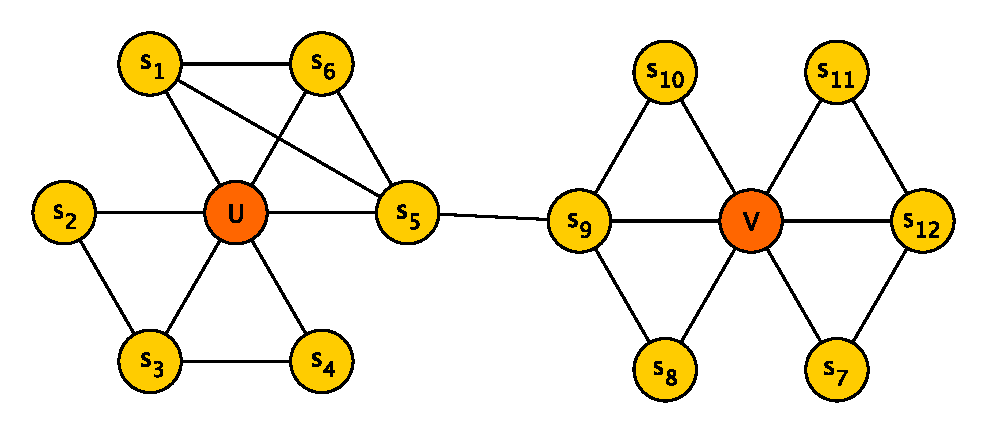
\includegraphics[width=0.5\textwidth]{images/Fig1.pdf}\\
	\caption{Nodes U and V are structurally equivalent; nodes V and s9 belong to the same community}
	\label{fig:Fig1}
\end{figure}

Consider a graph at the~\autoref{fig:Fig1}. A structural equivalence concept states that nodes U and V have the same structural role as a common connection mediating the short path lengths between other nodes. But at the same time, they belong to different communities unlike nodes V and $s_9$, that share the same community - a homophily concept. Due to the structural equivalence hypothesis, nodes U and V should be embedded closely together while nodes V and $s_9$ should be also embedded closely together due to the homophily hypothesis as they belong to the same community.

The unique sampling strategy of Node2vec uses a random walk approach in a graph. It is a stochastic process aimed to describe a path through the successive nodes linked by edges chosen at random. Such technique allows flexible neighbourhoods which can capture at some extent nodes’ structural equivalence along with homophily. The transitions from previous to the next node in a path simulated by random walk process obeys the following distribution law (parameters are explained in the~\autoref{tab:tab1}): 

\begin{equation}
  P(c_i=x | c_{i-1}=v) =
    \begin{cases}
      \frac{\pi_{vx}}{Z} & \text{if $(v,x) \in E$} \\
      0 & \text{otherwise}
    \end{cases}
    \label{eq:equat1}
\end{equation}

\begin{table}
\begin{center}
\begin{tabular}{ | m{1em} | m{2cm}| m{11cm} |} 
\hline
\textbf{\#} & \textbf{parameter} & \textbf{description} \\ 
\hline
1 & $G =(V,E)$ & graph of nodes $V$ and edges $E$ \\ 
\hline
2 & $d_{tx}$ & the shortest path distance between nodes $t$ and $x$ \\
\hline
3 & $l$ & walk length \\
\hline
4 & $u$ & source node \\
\hline
5 & $c_i$ & $i$-th node in the walk \\
\hline
6 & $\pi_{vx}$ & unnormalized transition probability between nodes $v$ and $x$ \\
\hline
7 & $Z$ & normalizing constant \\
\hline
8 & $w_{vx}$ & $vx$ edge weight (=1 for unweighted graphs) \\
\hline
\end{tabular}
\caption {Parameter descriptions}
\label{tab:tab1}
\end{center}
\end {table}

Nove2vec uses a slightly modified~\autoref{eq:equat1} introducing the bias parameter $\alpha$. Assume the random walk process has just transitioned from node $t$ to node $v$ in the~\autoref{fig:Fig2}, the probability to transition from $v$ to any one of its neighbours is $w_{vx} *\alpha$ (normalized), where:

\begin{equation}
  \alpha_{pq}(t,x) = 
    \begin{cases}
      \frac{1}{p} & \text{if $d_{tx}=0$} \\
      1 & \text{if $d_{tx}=1$} \\
      \frac{1}{q} & \text{if $d_{tx}=2$}
    \end{cases}
    \label{eq:equat2}
\end{equation}
\begin{figure}[!hp]
    \vspace{0pt}
    \centering
    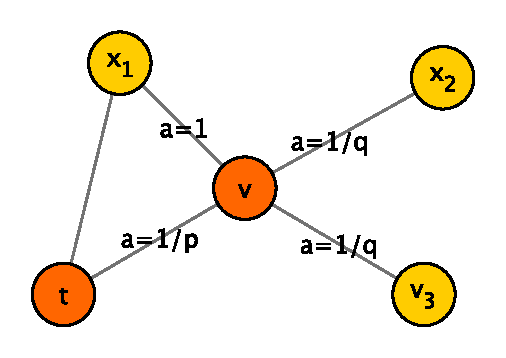
\includegraphics[width=0.4\textwidth]{Fig2.pdf}
    \caption{A random walk process has just traversed edge $(t,v)$. The probabilities of the next transit from $v$ to any node depend on the parameter $\alpha$}
    \label{fig:Fig2}
\end{figure}
As a shortest path $d_{tx} \in \{ 0, 1, 2 \} $ two parameters are sufficient to smoothly control a random walk: $q$ relates to a further neighbourhood exploration (transitions $(v, x_2), (v, x_3)$) and $p$ describes the likelihood of immediately revisiting a node in the walk (transitions $(v, t)$). Together they intuitively control the total speed of random walk in the network exploration in a way described in ~\autoref{tab:tab2}.
\begin{table}[!hp]
\begin{center}
\begin{tabular}{|c|c|c|}
    \hline
    Parameters & Value & Sampling intuitions \\
    \hline
    \multirow{2}{*}{Return parameter $p$} & $> max(q,1)$ & less likely to sample an already-visited node \\\cline{2-3}
    & $< min(q, 1)$ & keep the walk close to the source node \\
    \hline
    \multirow{2}{*}{In-out parameter $q$} & $> 1 $ & bias towards nodes close to source node \\\cline{2-3}
    & $< 1$ & bias towards nodes further away from source node \\
    \hline
\end{tabular}
\end{center}
\caption{Node2vec $p$ and $q$ parameters tuning}
\label{tab:tab2}
\end{table}
Essentially, the conditional transition probability $\pi_{vx}$ of the random walk process, given the present state and one state before, is a function of a preceding node $t$ in the walk ($t -> v -> x$), which makes the random walk a $2^{nd}$ order Markovian. 
The described above sampling algorithm for networks has effective time complexity $O(\frac{l}{k(l-k)})$ per sample~\cite{node2vec}, where a random walk of length $l>k$ can generate k samples for l−k nodes at once. Although a random partial sample reuse across different source nodes can shuttle it insignificantly. It is much better than the classic search-based sampling strategies like breadth-first sampling (BFS) and depth-first sampling (DFS)~\cite{node2vec}. 
The result of the sampling stage of Node2vec framework is a group of directed acyclic graphs generated from the input graph $G(V,E)$. Each of these graphs is a stochastic representation of the node’s neighbourhood. An analogy in NLP would be a text sentence where each word is a node and all words follow a certain order.

\textbf{Limitations. } 
\label{Limitations of Node2vec}
However, the usage of a random walk for sampling exposes some limitations. The set of learned features is unable to transfer to new nodes and graphs as they are tied to vertex identity. Furthermore, the structural hypothesis fails when nodes with similar neighbourhood structures are located within different graph components or sufficiently far from each other. The random walk sampling captures mostly proximity of the nodes in a graph rather than a structural similarity of their neighbourhoods. Goyal and Ferrara demonstrated it in their recent paper ~\cite{Goyal2018GraphET}. This comprehension comes from the fact that nodes are uniquely identified within a graph. Thus, two node embeddings will be placed closer to each other in a low-dimensional space if they have been derived from two overlapping random walk samples, precisely speaking - two samples that have a portion of the same nodes. These flaws and one of the possible solutions have been discussed in 2018 by Nesreen K. Ahmed et al.~\cite{role2vec}. 

\subsubsection{Skip-gram model}
\label{Skip-gram_Model}
At the next stage, the Node2vec framework like some other recent network embedding frameworks ~\cite{perozzi2014deepwalk}, ~\cite{tang2015line} uses a widely known Skip-gram model~\cite{SKIP-GRAM-MODEL} that came from NLP in order to learn continuous feature representations from gathered samples. The model was originally introduced by T. Mikolov et al. in ~\cite{SKIP-GRAM-MODEL} and initially served for learning vector representations of words in a text by optimizing a neighbourhood preserving likelihood objective. Later, it was adapted for feature learning in networks. The core principles of skip-gram model for network embedding will be discussed below.

\textbf{Model objective. }The skip-gram language model is an efficient method for learning high-quality vector representations of words from large amounts of unstructured text data. Specifically, skip-gram maximizes the co-occurrence probability among the words that appear within a window $w$ in a sentence. This intuition came from a hypothesis stated in 1954 by Zellig S. Harris that each language can be described in terms of a distributional structure~\cite{Zellig:DistributionalStructure}. It claims that words in similar contexts tend to have similar meanings, namely words tend to appear in similar contexts.
The~\autoref{fig:Fig3} represents the random walk paths for each node in a graph as a sampling result from \ref{Sampling strategy} where nodes constitute a vocabulary to train the skip-gram model.
\begin{figure}[!hp]
    \centering
    \begin{minipage}{0.45\textwidth}
        \centering
        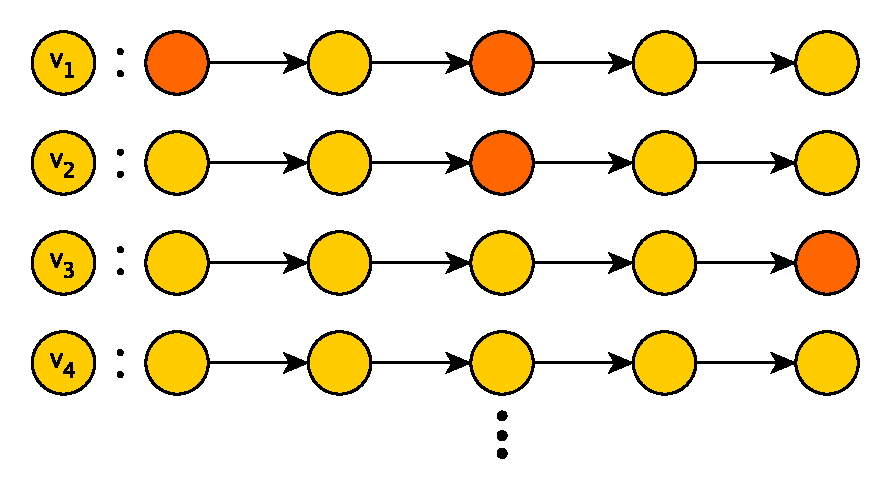
\includegraphics[width=0.9\textwidth]{Fig3.pdf}
        \caption{A group of the directed acyclic graphs sampled from an underlying network}
        \label{fig:Fig3}
    \end{minipage}\hfill
    \begin{minipage}{0.45\textwidth}
        \centering
        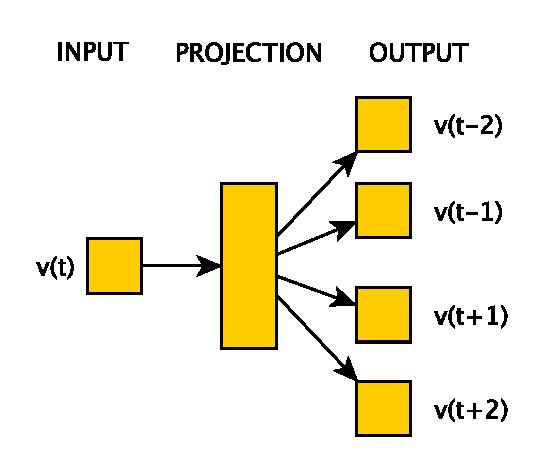
\includegraphics[width=0.9\textwidth]{Fig4.pdf} 
        \caption{Skip-gram model predicts surrounding nodes given the current node}
        \label{fig:Fig4}
    \end{minipage}
\end{figure}
A precise aim of the skip-gram as described in~\cite{SKIP-GRAM-MODEL} is to predict surrounding nodes given a current node. It is achieved by inputting each current node to a log-linear classifier with continuous projection layer, and by predicting nodes within a certain range before and after the current node~\autoref{fig:Fig4}.
Predictions are based on a node proximity to the source node within the sampling graph: more distant nodes get less weight, since they are usually less related to the source node (important: a sampling graph may include a source node more than once in different positions). It is worth to mention that an increasing range of prediction (the length of sample graphs) improves the resulting quality of node representations but at the same time increases computational complexity.
The algorithm estimates continuous representations of nodes by means of recurrent neural network (RNN). The current RNN model architecture was firstly proposed by Tomas Mikolov et al. in 2010 and later described in~\cite{mikolov2013linguistic} in the context of learning continuous word representations. Its adapted version for the network embeddings learning problem is illustrated in~\autoref{fig:Fig5}.

\begin{figure}[H]
    \centering
    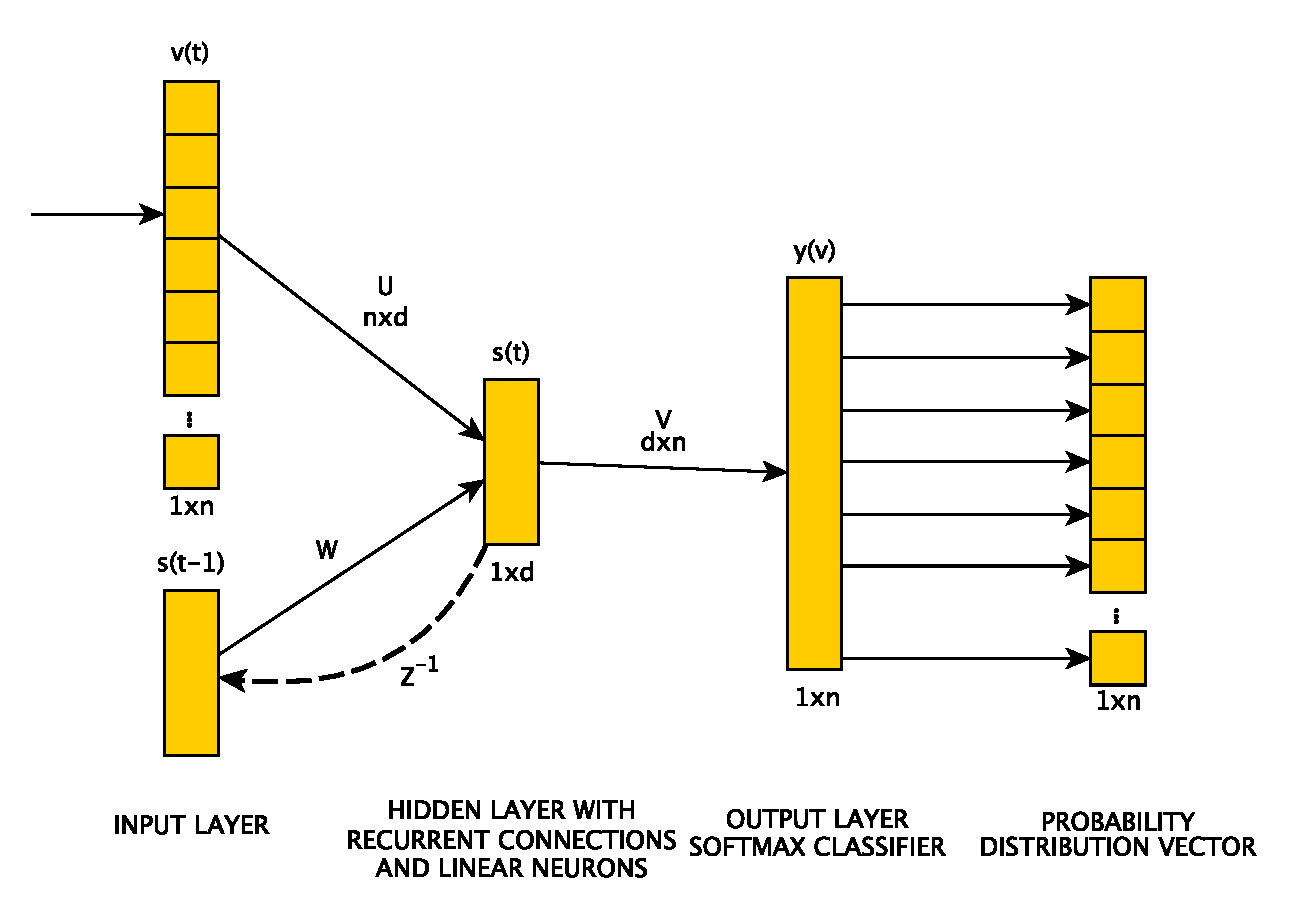
\includegraphics[width=0.7\textwidth]{Fig5.pdf}
    \caption{RNN architecture}
    \label{fig:Fig5}
\end{figure}
\begin{figure}[H]
    \centering
    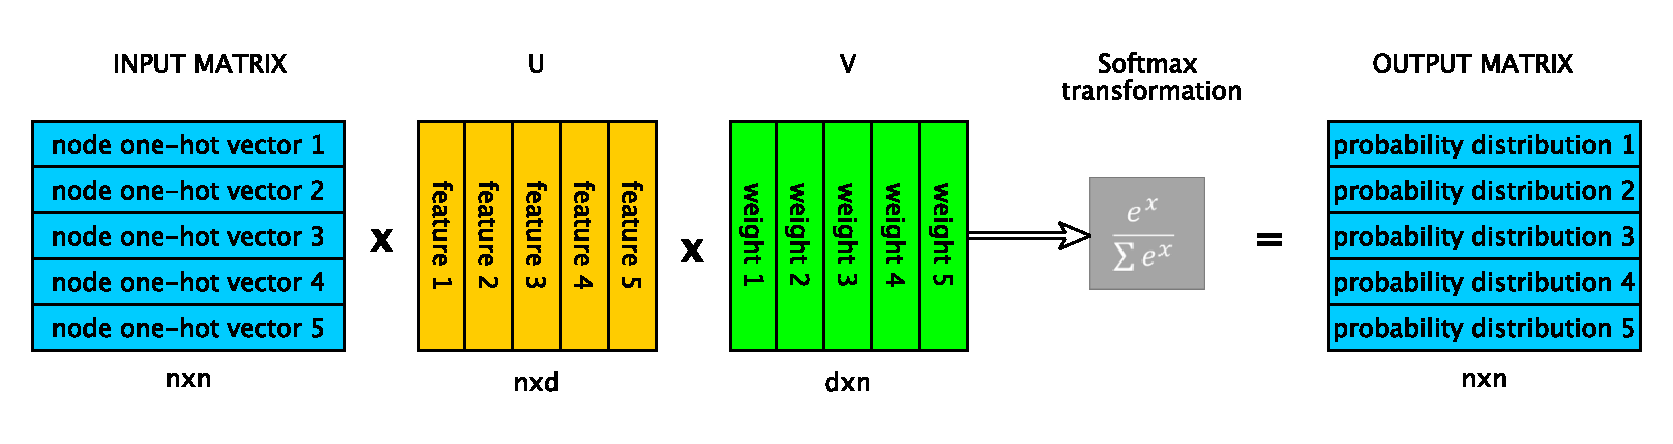
\includegraphics[width=0.7\textwidth]{Fig6.pdf}
    \caption{Probability vectors generation in a matrix notation}
    \label{fig:Fig6}
\end{figure}

Vector $v(t)$ represents an input node at time $t$ encoded using one-hot encoding (vector has “1” in the source node position and “0” in other positions). Vector $v$ has $n$ components, where $n$ is equal to the number of nodes in the underlying network. The output vector $y(v)$ of size $n$ produces a probability distribution over nodes in a network. A hidden layer has $d$ neurons and maps each input vector to its current representation maintaining it over time $t$ by maximizing the probability of source node’s neighbours:
\begin{equation}
  \textbf{s}(t) = f(\textbf{Uw}(t) + \textbf{Ws}(t-1))
    \label{eq:equat3}
\end{equation}
There is no activation function in the hidden layer neurons, and each neuron has a weight vector stored in $\textbf{V}$. Node vectors from the hidden layer $s(t)$ are multiplied with the weight vectors from $\textbf{V}$ and then are subjected to Softmax regression classifier. The last transformation is responsible for each output vector summing up to 1, as they represent some probability distributions. The result from neurons in the output layer is calculated as follows:
\begin{equation}
  \textbf{y}(t) = g(\textbf{Vs}(t)),\;\;\;
  where \;\; f(z)= \frac{1}{1+e^{-z}},\;\;\; g(z_m)=\frac{e^{z_m}}{\sum\limits_{j=1}^n e^{z_j}}
\label{eq:equat4}
\end{equation}
However Softmax classifier at the last step doesn't scale on very large networks. One solution of this problem is "Negative sampling", which will be discussed in \ref{Model training} subsection. ~\autoref{fig:Fig6} illustrates the calculations in a matrix notation. 

Once the RNN is trained via back-propagation, it is not supposed to be used directly for the task it has been trained. Instead, the goal is to learn the hidden layer weight matrix $\textbf{U}$. The columns of the $U$ matrix are the sought-for node representations.

\textbf{Model training. }
\label{Model training}
The described RNN is intended to take a high-dimensional one-hot node vector as an input and output the respective probability distribution as shown in~\autoref{fig:Fig7}.
To train the skip-gram network, one needs to supply it with training example and slightly adjust weights for all neurons in a way that it predicts training sample more accurately. The ultimate prediction task is given a source node to predict the probability for every node in the vocabulary being close to the source. ~\autoref{fig:Fig8} shows how training examples extracted from an underlying network are converted to distribution vectors.

\begin{figure}[H]
    \centering
    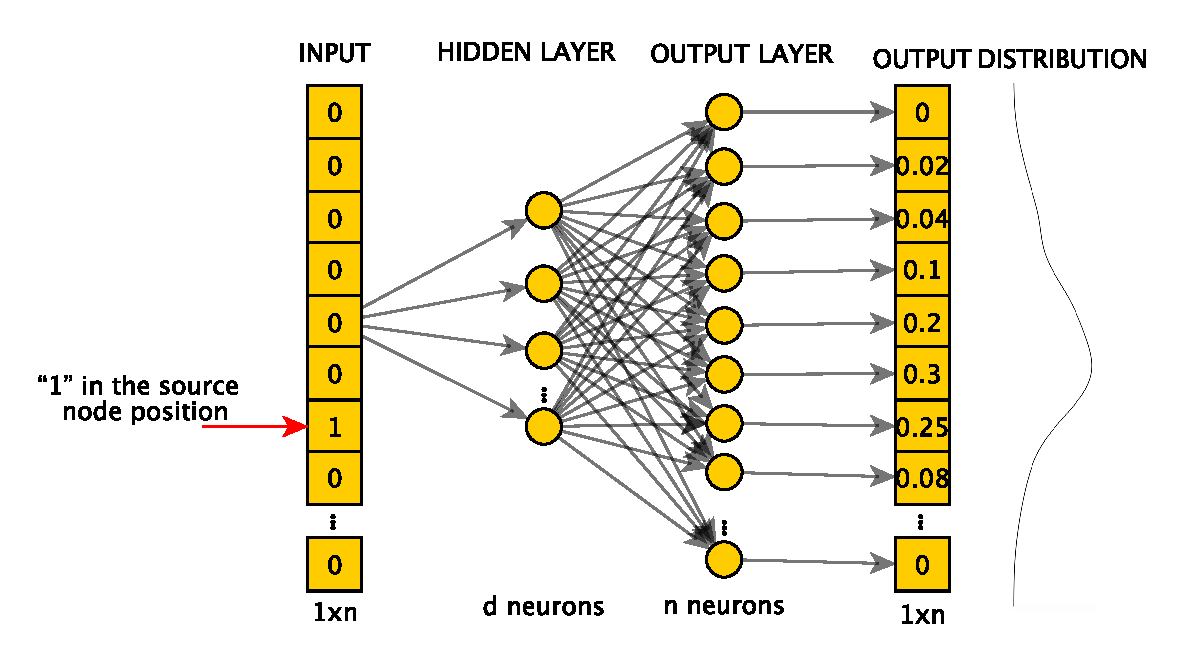
\includegraphics[width=0.7\textwidth]{Fig7.pdf}
    \caption{A group of the directed acyclic graphs sampled from an underlying network}
    \label{fig:Fig7}
\end{figure}
\begin{figure}[H]
    \centering
    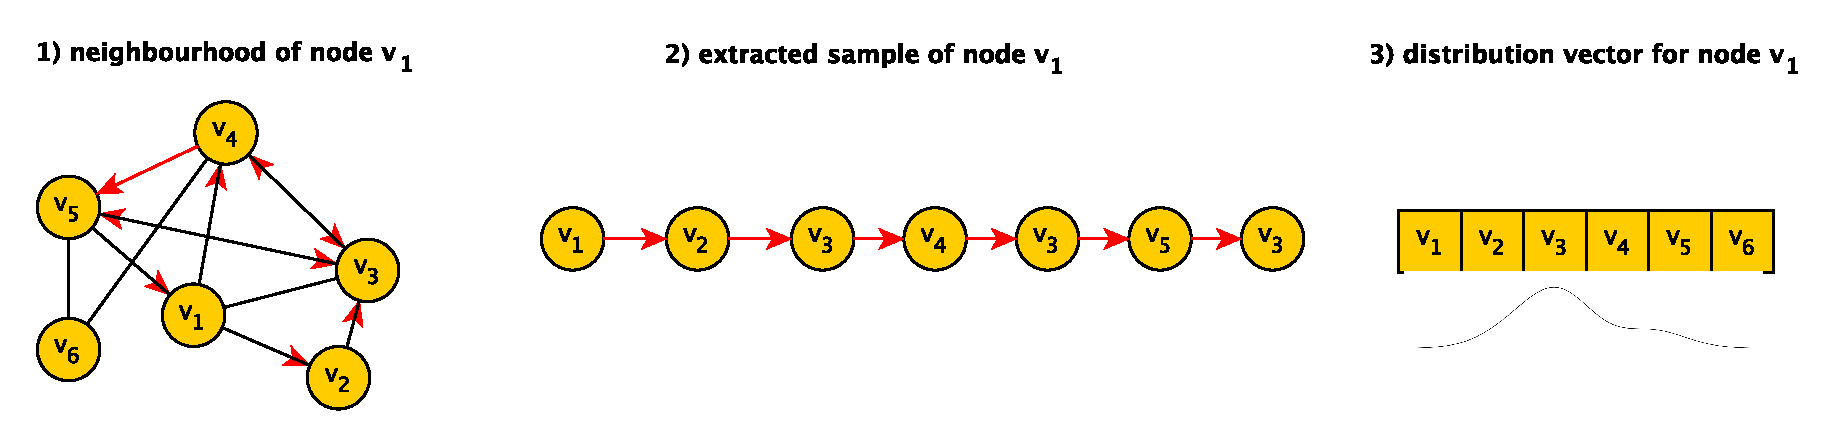
\includegraphics[width=0.7\textwidth]{Fig8.pdf}
    \caption{Skip-gram model predicts surrounding nodes given the current node}
    \label{fig:Fig8}
\end{figure}

Unfortunately, the direct model training for large networks of size $n$ and the number of hidden layer neurons $d$ is in general computationally inefficient as it has to generate $2*n*d$ weights for the hidden and output layers. At the same time, it requires an immense amount of training data to generate all the weights and avoid running into over-fitting. 
To facilitate the training process Mikolov et al. proposed a “Negative sampling” (NEG) in~\cite{gutmann2012noise}. This technique makes the training feasible. The intuition behind is to sample only $k$ negative nodes (negative nodes are those whose one-hot vector has 0 at the source node position) according to some noisy distribution $P_n(v)$ for each source node vector and modify only some weights rather than all of them. Applying NEG the SoftMax objective~\autoref{eq:equat4} transforms into a new one:
\begin{equation}
  \log{f(z_m)} + \sum\limits_{i=1}^k \mathbb{E}_{v_i\sim P_n(v)} [\log{f(z_i)}],\;\; 
  where \;\; f(z)= \frac{1}{1+e^{-z}}
    \label{eq:equat5}
\end{equation}

Running an asynchronous stochastic gradient descend on this modified objective speeds up the training process dramatically what was experimentally shown in~\cite{Mikolov:Word2vec}. Additionally, in this paper Mikolov et al. discussed the choice of $k$ – number of negative samples and $P_n(v)$ – node-specific distribution. In general, for large networks $k$ is supposed fluctuating from 2 to 5 negative node-vectors, drawn from $P_n(v)$ - a unigram term frequency distribution.

\begin{figure}[H]
    \centering
    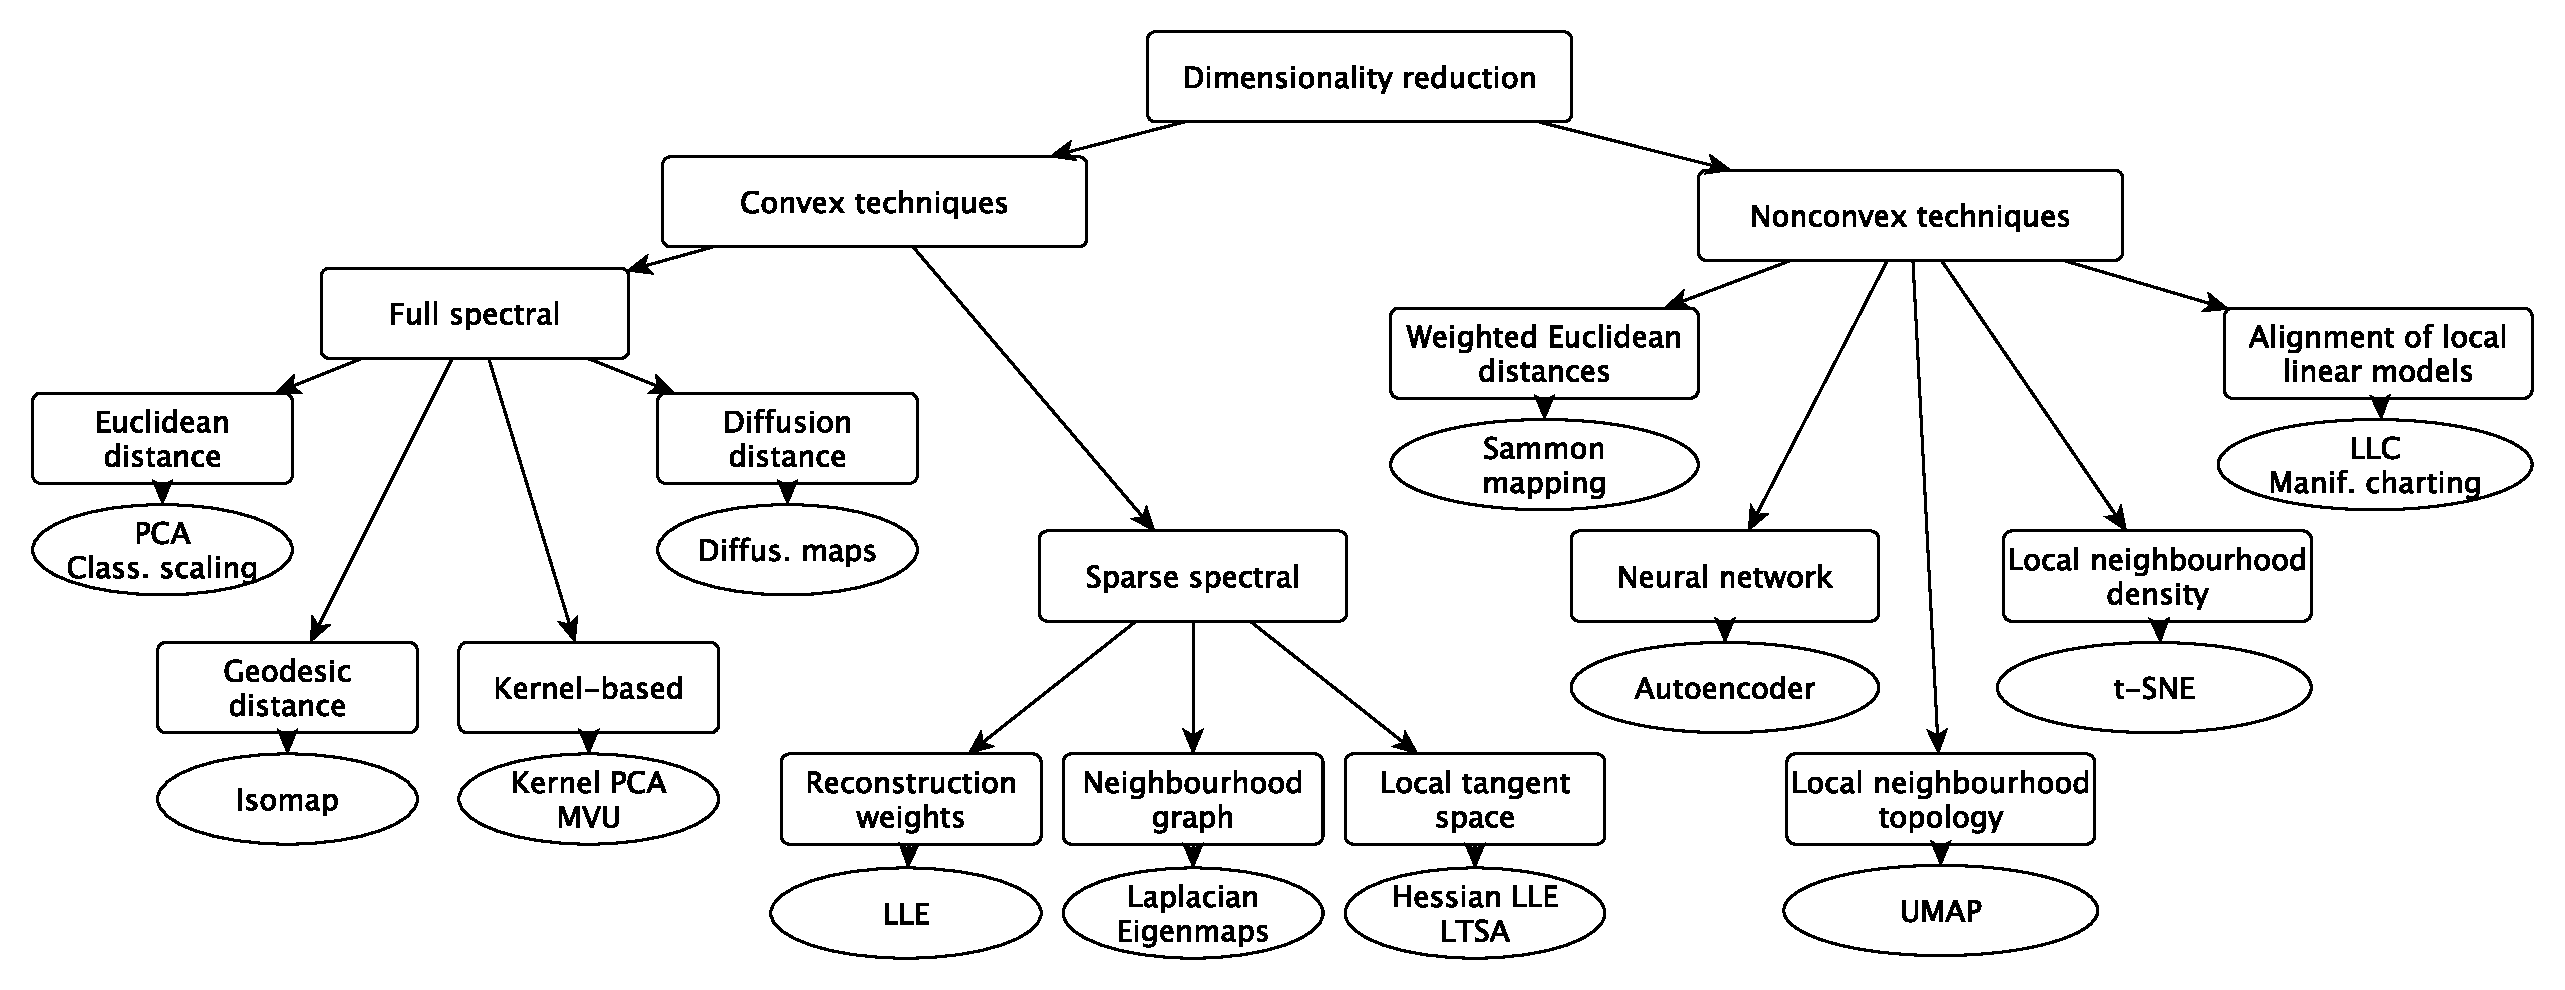
\includegraphics[width=1.0\textwidth]{Fig10.pdf}
    \caption{Taxonomy of dimensionality reduction techniques}
    \label{fig:Fig10}
\end{figure}

\section{Dimensionality Reduction}
\label{Dimensionality Reduction}
Dimensionality reduction is the transformation of high-dimensional data into a meaningful representation of reduced dimensionality. In the ideal case, a reduced representation should have a dimensionality equal to the data intrinsic dimensionality what means a minimum number of parameters needed to account for observed properties of the data. Dimensionality reduction is important to this work as it mitigates the "curse of dimensionality" which naturally occurs in high-dimensional feature space learned from a network at the previous pipeline stage.

~\autoref{fig:Fig10} exhibits an extended taxonomy of techniques for dimensionality reduction inspired by~\cite{van2009dimensionality}. The upper subdivision into convex and non-convex techniques comes from the objective function that has to be optimized. A convex techniques' objective function does not contain a local optima in the convex solution space and can be optimized by solving a generalized eigenproblem. The further subdivision of convex techniques is based on the performance of an eigendecomposition of a full matrix or a sparse matrix. An objective functions of non-convex techniques do contain local optima. The extensive overview of all techniques mentioned in the taxonomy could be found in ~\cite{van2009dimensionality}.

\subsection{Principal Components Analysis}
Although in the last decades many nonlinear dimensionality reduction techniques have been proposed, the linear PCA remains the most popular unsupervised method because of its simplicity and solid result interpretability. It transforms linearly the original input which is typically high-dimensional into new uncorrelated features. The ultimate goal is to find a low-dimensional representation of the data preserving as much of the variance in the input data as possible. The PCA became of great demand in machine learning as it cleans up the data from extraneous variables which in fact contain little information. Thus, it allows to speed up perceptibly machine learning algorithms performance at the cost of accuracy. Finally, another major application scenario of PCA is data visualization. It allows approximate visualization high-dimensional data in 1D, 2D or 3D space by taking the axes along the directions of the highest variances in the data. The concept consists of several steps, which will be described below.

\textbf{Concept. }
The first step of PCA is a standardization of the input data, what means to subtract from each feature its mean and divide by its standard deviation. The second step is to obtain the basis of orthogonal eigenvectors and spectrum from the covariance matrix of standardized data. The next is sorting the calculated eigenvalues in descending order and consider the first $k < n$ where $k$ is a desired number of dimensions and $n$ is dimensionality of the original space. After, construct the projection matrix from the eigenvectors that correspond to the chosen ordered $k$ eigenvalues. Finally, to obtain the new representation of the data in the reduced $k$-dimensional space transform the original data set by multiplying it by the projection matrix.
In mathematical terms, PCA solves the standard eigenproblem for covariance matrix in case of standardized data~\autoref{eq:equat6} (for correlation matrix in case of non-standardized data).

\begin{equation}
  cov(\textbf{X})\textbf{M} = \lambda \textbf{M}
    \label{eq:equat6}
\end{equation}

where $cov(\textbf{X})$ is the sample covariance matrix of the standardized data $\textbf{X}$ and $\textbf{M}$ is the linear basis of eigenvectors. The trick allows to reduce the output space in matrix $\textbf{M}$, that consists of the $k$ eigenvectors corresponded to the largest eigenvalues of the $cov(\textbf{X})$. Thus, the sought-for low-dimensional data representation is 

\begin{equation}
  \textbf{Y} = \textbf{X}\textbf{M}
    \label{eq:equat7}
\end{equation}

\textbf{Limitations. }The fact that nowadays the linear PCA remains at the peak of popularity among dimensionality reduction techniques in machine learning after more than a century from its first formulation by Karl Pearson proves its ubiquitous practical value. Nevertheless, a comparative review of dimensionality reduction techniques from 2009 ~\cite{van2009dimensionality} shows that nonlinear techniques outperform linear techniques on selected data sets that typically contain well-sampled smooth manifolds. But that does not guarantee anything regarding the real-world data. In fact, they show that most nonlinear techniques do not outperform linear PCA on natural data sets. 
In general, full spectral linear dimensionality reduction techniques like PCA suffer from the inability of modelling complex nonlinear manifolds. This idea has been clearly illustrated by Laurens van der Maaten in ~\cite{maaten2008visualizing} on a toy example - a “Swiss roll” data set ~\autoref{fig:Fig11}. This necessitates a search for other intuitions unlike preserving large pairwise distances to maximize variance like PCA does. Another drawback concerns the information loss: a new representation of the data will no longer contain the information from those features that have been excluded.

\begin{figure}[H]
    \centering
    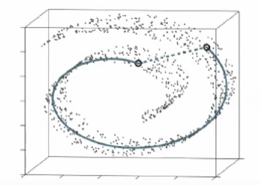
\includegraphics[width=0.5\textwidth]{Fig11.png}
    \caption{A Swiss Roll data set plotted in 3D space. PCA will fail to find non-linear circular path. Data source: http://people.cs.uchicago.edu/~dinoj/manifold/swissroll.html}
    \label{fig:Fig11}
\end{figure}

\subsection{t-Distributed Stochastic Neighbour Embedding}
t-Distributed Stochastic Neighbour Embedding is an unsupervised nonlinear dimensionality reduction technique that aims to preserve the local structure of data in a visualization task. It has been initially proposed by Laurens van der Maaten and Geoffrey Hinton in~\cite{maaten2008visualizing} as an optimisation of stochastic neighbour embedding ~\cite{hinton2003stochastic} to overcome its main flaw - an excessive crowding of objects while mapping them to low-dimensional space. L. van der Maaten and G. Hinton compared in their study seven most known nonlinear techniques against t-SNE and revealed that t-SNE outperforms others in visualisation of a MNIST data set \footnote{The MNIST data set contains 60,000 grayscale training images of handwritten digits and is publicly available from http://yann.lecun.com/exdb/mnist/index.html} and separates objects of different digits better than other techniques.
The t-SNE concept on a high level looks as follows: the algorithm calculates two similarity measures between pairs of instances in a high dimensional space and in low dimensional space and tries to optimize them using a cost function.

\textbf{Concept. }~\autoref{fig:Fig12} shows some points in a high dimensional space. To measure similarities between these points, t-SNE centres a Gaussian over a point $x_i$ and consider its local neighbourhood. Instead of calculating all pairwise distances between points like full spectral techniques do, t-SNE measures only local distances to nearby points. A conditional probability density function $p$ describes the probability of two points being close to each other and is constructed as follows:

\begin{equation}
  p_{j|i}=\frac{\exp{(-||x_i-x_j||^2/2\sigma_{i}^2)}}{\sum_{j`\neq i}\exp{(-||x_i-x_j`||^2/2\sigma_{i}^2)}}
    \label{eq:equat8}
\end{equation}

\begin{figure}[H]
    \centering
    \begin{minipage}{0.45\textwidth}
        \centering
        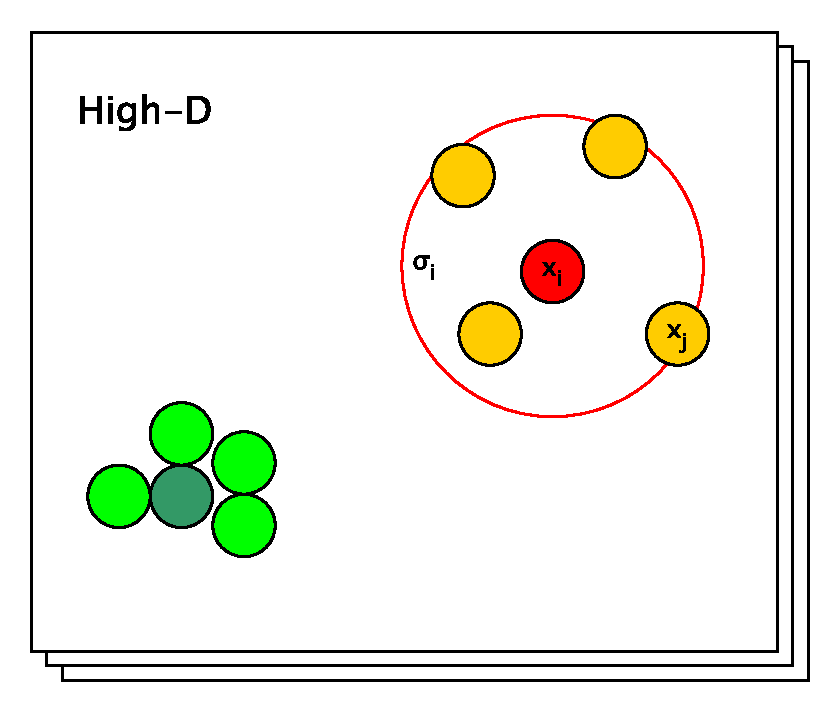
\includegraphics[width=0.9\textwidth]{Fig12.pdf}
        \caption{Points in a high dimensional space are not equally distributed. Perplexity parameter of t-SNE is responsible to scale bandwidth $\sigma_i$ to consider a roughly fixed number of points within each Gaussian.}
        \label{fig:Fig12}
    \end{minipage}\hfill
    \begin{minipage}{0.45\textwidth}
        \centering
        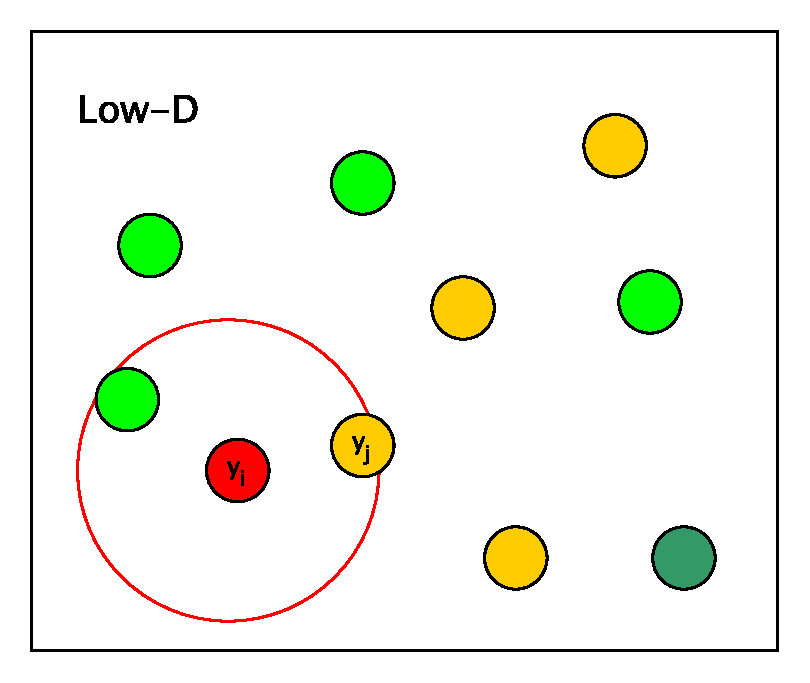
\includegraphics[width=0.9\textwidth]{Fig13.pdf} 
        \caption{Initial representations of points from a high-D space in a low-D space. The discrepancies between pairwise distances in a high-D and low-D are optimized by the gradient of the objective function.}
        \label{fig:Fig13}
    \end{minipage}
\end{figure}

$x_i$ is the fixed centre of the Gaussian and $x_j$ are other points under this gaussian. The bottom part of the equation is a normalization factor specific to this particular Gaussian that normalizes probabilities over pairs that involves point $x_i$. This way of normalization allows to set a different bandwidth of $\sigma_i$ for each point and thereby fix perplexity for the conditional distribution. ~\autoref{fig:Fig12} demonstrates the scaling of the bandwidths of the Gaussians depending on the number of points falls into the Gaussians. Points in the original space are typically distributed nonuniformly and this scaling technique enables to adapt to different densities.
The further assumption is the final joint probability $p_{ij}$ is a summarized average of the conditional probabilities $p_{j|i}$ and $p_{i|j}$:

\begin{equation}
  p_{ij}=\frac{p_{j|i} + p_{i|j}}{2N}
    \label{eq:equat9}
\end{equation}

In fact, the probability $p_{ij}$ is proportional to the similarity of points $x_i$ and $x_j$. A large magnitude for $p_{ij}$ signalizes two points $x_i$ and $x_j$ are close together in the original high-dimensional space and infinitely small $p_{ij}$ implies two points are far apart.
The next step is to build low-dimensional representations for each point from the high-dimensional space. Assume these representations are on the ~\autoref{fig:Fig13}. To come up with the similar probabilistic measure of points similarities, construct a function with a kernel distribution centered in $y_i$:

\begin{equation}
  q_{ij}=\frac{(1+||y_i-y_j||^2)^{-1}}{\sum_{k}\sum_{l\neq k}(1+||y_k-y_l||^2)^{-1}}
    \label{eq:equat10}
\end{equation}

the bottom part here is a normalization factor over all pairs of points in the low-D space. The probability $q_{ij}$ measures the similarity of $y_i$ and $y_j$. 
The ultimate goal of the algorithm is to minimize the difference between two probability functions $p$ and $q$ in a way that $q$ is a reflection of the ground truth $p$. A common measure of entropy - Kullback–Leibler divergence is used for this purpose:

The KL criterion is a "distance measure" of two probability distributions that is necessary to be minimized over all pairs of points via gradient descent for the current task. The asymmetry of the KL divergence facilitates to preserve local structure of points in the high-D space. Assume that $x_i$ and $x_j$ are close together and thus $p_{ij}$ value is large. In order to minimize the sum of the KL divergences in the ~\autoref{eq:equat11} the $q_{ij}$ has to be also a large value. That means that the corresponding points $y_i$ and $y_j$ in the low-D are also close together. Overall, the optimizing procedure of the KL divergences tries to model large values of $p_{ij}$ by corresponding large values of $q_{ij}$. Although, because of the asymmetry of the KL divergence, it does not guarantee the same for the inverse case: if two points are very dissimilar (small $p_{ij}$), then the corresponding contribution to the sum is very small and by this irrelevant regardless of a $q_{ij}$ value. This fact enables t-SNE to capture local structures of a high-D space.

One of the crucial enhancements over the antecedent Stochastic neighbour embedding approach (SNE) ~\cite{hinton2003stochastic} is a usage of Student t-distribution with one degree of freedom instead of normal for $q$ in the ~\autoref{eq:equat10}. ~\autoref{fig:Fig14} demonstrates the clear difference in the shapes of two distributions. Student t-distribution is a lot more heavy-tailed compared to a Gaussian. Assume the probability $q_{ij}$ is low and points $y_i$ and $y_j$ are dissimilar. Because of using a heavy-tailed distribution the points will be placed too far apart from each other and thereby will not crowd around the centre. The crowding problem of SNE under the Gaussian distribution has been clearly described in ~\cite{maaten2008visualizing}.

\begin{equation}
  C = \sum_{i}KL(P_i||Q_i)=\sum_{i}\sum_{i\neq j}p_{ij}\log{\frac{p_{ij}}{q_{ij}}}
    \label{eq:equat11}
\end{equation}

\begin{figure}[!hp]
    \centering
    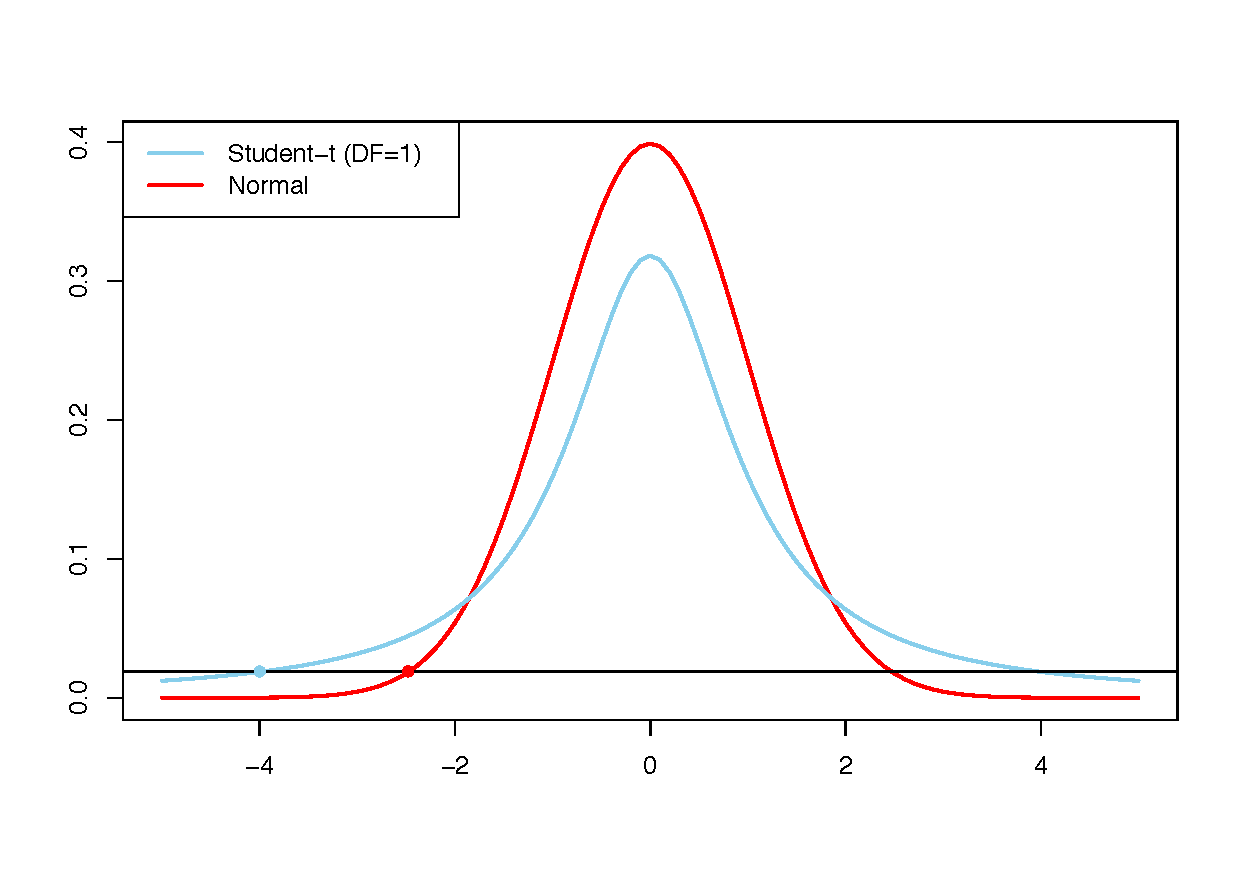
\includegraphics[width=0.5\textwidth]{Fig14.pdf}
    \caption{Heavy-tailed distribution allows two dissimilar points to be far apart from each other in the projected low-D space, as on the same low value of probability (referencing dissimilar points), the Student t-distribution places two points further apart.}
    \label{fig:Fig14}
\end{figure}

\textbf{Model objective and optimization. }
As mentioned above the cost function of t-SNE is a sum of Kullback–Leibler divergences which optimized by gradient descent. The gradient of the KL divergence between the Gaussian distribution $P$ and the Student t-distribution $Q$ with respect to a point is given by:

\begin{equation}
  \frac{\partial C}{\partial y_i}= 4\sum_{j\neq i}\underbrace{(p_{ij}-q_{ij})(1+||y_i-y_j||^2)^{-1}}_\text{I}\underbrace{(y_i-y_j)}_\text{II}
    \label{eq:equat12}
\end{equation}

The transformation of ~\autoref{eq:equat12} into ~\autoref{eq:equat11} is covered in Appendix A of ~\cite{maaten2008visualizing}. The second part of the gradient (II) is a directed spring between pair of nodes and the first part (I) measures an exertion of this spring based on the difference between $p_{ij}$ and $q_{ij}$. This difference is equal to zero if $q_{ij}$ models $p_{ij}$ perfectly. The optimization process is moving points around the fixed one at each step until to attain a lower KL divergence.
A computation of t-SNE representations outperform SNE as a Student t-distribution does not involve an exponential unlike a Gaussian and thereby density evaluation of a point is faster.

\textbf{Limitations. }
As gradient of the model objective considers all pairwise interactions between points, having $n$ points the $n^2$ interactions between them have to be considered and sum in every gradient update. This limits a t-SNE application to 5 000 - 10 000 points in a space. This restriction could be mitigated applying Barnes-Hut approximation ~\cite{Barnes1986}: instead of calculating every pairwise distance, group points together where possible to calculate one distance between point and group of points.
Another major weakness of t-SNE is in its nonconvex cost function. An output solution is stochastic and depend on optimization parameters. It may vary each t-SNE run even preserving the same set of optimization parameters, however, the quality of the optima does not change much from run to run.
t-SNE fails to preserve pairwise distances on a global structural level. On the  ~\autoref{fig:Fig15} two Gaussians with scaling bandwidths $\sigma_i$ and $\sigma_j$ are centered at $x_i$ and $x_j$. The respective conditional probabilities are evidently $p_{j|i} > p_{i|j}$ under a perplexity optimization parameter. The final joint probability $p_{ij}$ is the average of conditionals for two points viewed within their local neighbourhoods. Thereby the resulting probability $p_{ij}$ may not reflect the true pairwise distance on a global structural view and points' counterparts in the low-D will not globally preserve relevant distances. It follows that, in general, t-SNE does not preserve either distances nor density of the original space, it aims to reflect the structures observed in the high-D space by learning local neighbourhoods of points. 

\begin{figure}[!hp]
    \centering
    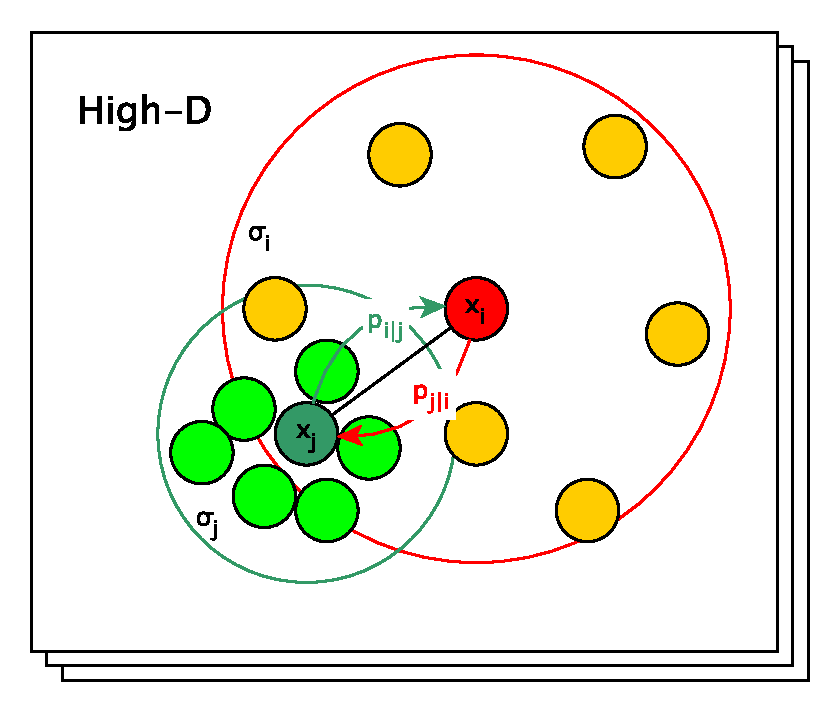
\includegraphics[width=0.5\textwidth]{Fig15.pdf}
    \caption{Example of the points distribution in a high-dimensional space when t-SNE mapping fails to preserve pairwise distance.}
    \label{fig:Fig15}
\end{figure}

t-SNE does not guarantee to reflect the same density clusters present in the original space, therefore density based algorithms should be applied on a t-SNE output with forethought, caution, and understanding the consequences or replaced by other techniques. Authors promote the technique as being well suited for data exploration and visualizing high-dimensional data, however conducting cluster analysis on t-SNE output is quite common in practice.

\subsection{Uniform Manifold Approximation and Projection}
One of the most recent technique from 2018 for dimensionality reduction is Uniform Manifold Approximation and Projection (UMAP). It is a competitor of t-SNE for visualization quality, and according to its creators, it preserves more of the global structure of the original data ~\cite{mcinnes2018umap}. Unlike t-SNE, UMAP has been presented as a dimension reduction technique for machine learning of general purpose.
Umap operates on Riemannian Manifolds and is able to recognize dense structures of arbitrary shape. It is faster than t-SNE, can handle larger high dimensional data sets, is able to scale well and better preserves a global structure of the data. 
The general idea behind UMAP is similar to t-SNE: construct two topological representations from the original high dimensional data and from some low dimensional representation and minimize the cross-entropy between the two topological representations. 

Assume some topological spaces constricted out of simple combinatorial components - simplices\footnote{\textbf{Simplex} - a generalization of the notion of a triangle or tetrahedron to arbitrary dimensions. Source: www.wikipedia.org}. A k-dimensional simplex (k-simplex) is formed by covering $k+1$ independent points by convex hull. On ~\autoref{fig:Fig17} each k+1-simplex consists of several k-simplices. This structural nesting allows generalization of topological spaces to arbitrary dimensions.

\begin{figure}[!hp]
    \centering
    \begin{minipage}{0.45\textwidth}
        \centering
        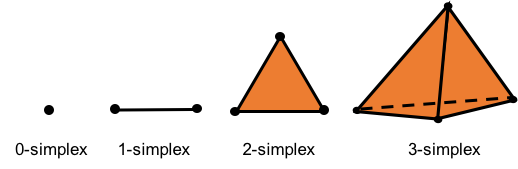
\includegraphics[width=1.2\textwidth]{Fig17.png}
        \caption{Low dimensional simplices.}
        \label{fig:Fig17}
    \end{minipage}\hfill
    \begin{minipage}{0.45\textwidth}
        \centering
        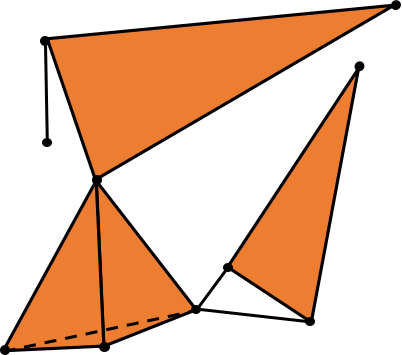
\includegraphics[width=0.45\textwidth]{Fig16_1.png} 
        \caption{Three-dimensional simplicial complex.}
        \label{fig:Fig16}
    \end{minipage}
\end{figure}

A simplicial complex on ~\autoref{fig:Fig16} is glueing together k-simplices along their faces (a dot is a face of 0-simplex, an edge is a face of 2 q-simplex, etc.). It serves for constructing topological spaces out of simplices of various dimensions~\cite{gamelin1999introduction}.
The goal is to cover finite sets of data points from Euclidean topology in a high-dimensional space by a simplicial complex. For this purpose, one can use open cover\footnote{\textbf{Open cover} - a collection of open sets of a topological space which union contains a given subset. For example, an open cover of the real line, with respect to the Euclidean topology, is a set of all open intervals (-n,n), where n in N. Source: http://mathworld.wolfram.com} to cover all sets in space. A Čech complex~\cite{MR1867354} provides a combinatorial way to convert open cover into a simplicial complex in the following simplified way: assume each set in the cover to be a 0-simplex, a 1-simplex is built between two such intersected sets, a 2-simplex spans three of such sets if their triple intersection is non-empty, etc. A solid mathematical justification of this process producing the meaningful topological space firstly has been formulated by K.Borsuk in 1948~\cite{Borsuk1948}, reviewed and proved later in many sources including ~\cite{MR1867354}, and nowadays is referenced as the Nerve theorem.
To learn about the topology of original space, one generates an open cover of it. To approximate an open cover, one can cover each point from the original finite set in a metric space with spheres of radius r. The process of learning a simplicial complex from the metric space is formally depicted on ~\autoref{fig:Fig18}.

\begin{figure}[!hp]
    \centering
    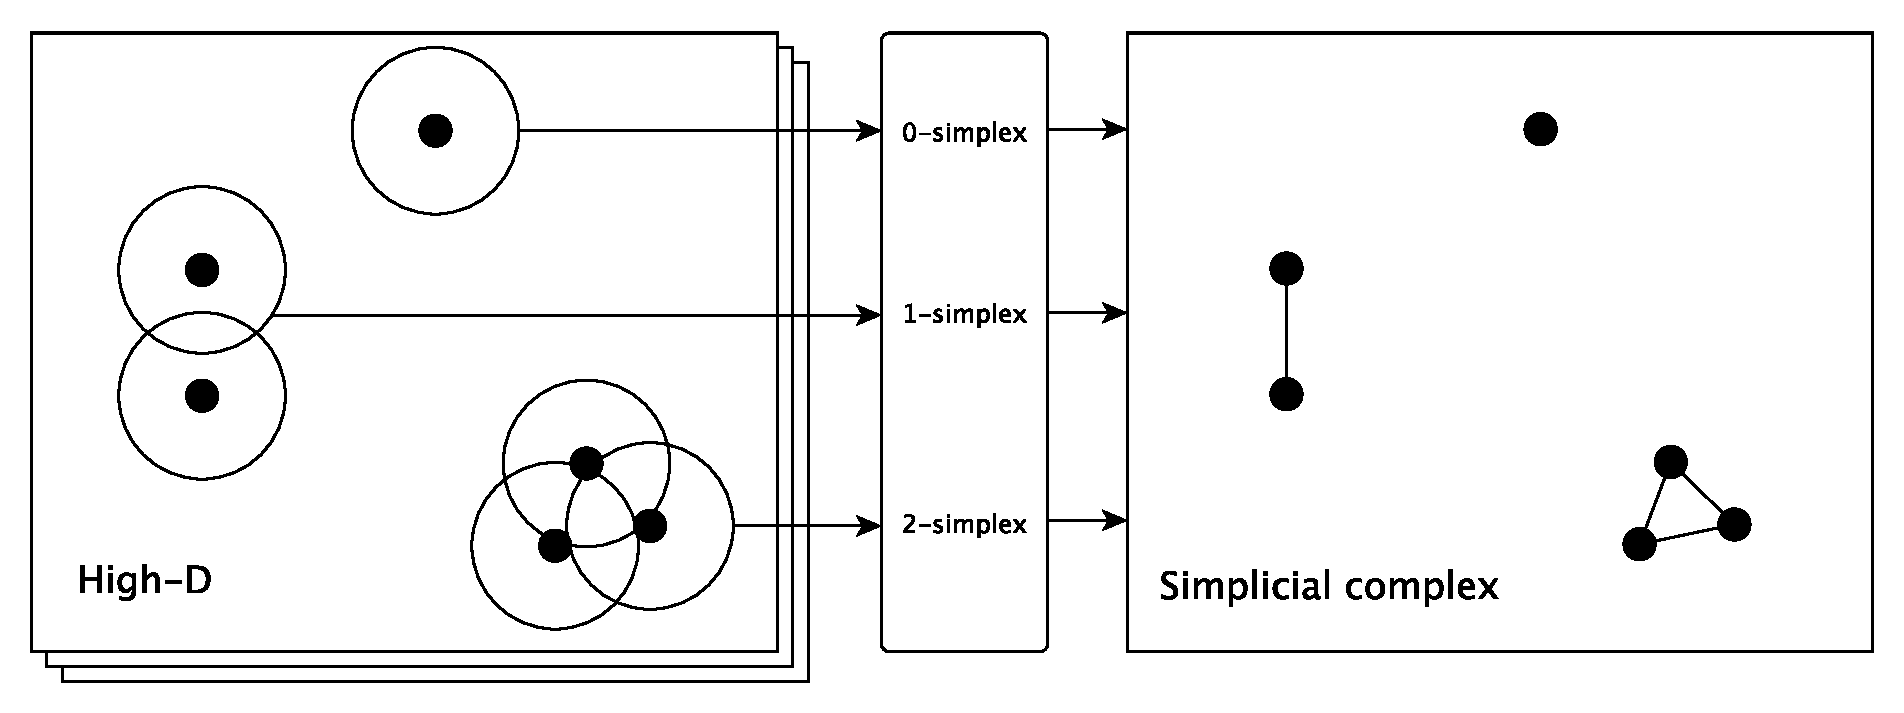
\includegraphics[width=0.8\textwidth]{Fig18.pdf}
    \caption{Process of learning a simplicial complex.}
    \label{fig:Fig18}
\end{figure}

Authors of the UMAP paper~\cite{mcinnes2018umap} proved that a simplicial complex indeed captures the fundamental topology better other approaches used by competitors like t-SNE. From the topological representation one can farther build a low dimensional representation for the data of similar topological representation. 
One of the toughest practical challenges is to come up with the right radius r of the spheres in an open cover approximation process~\autoref{fig:Fig18}. The precise math-justified way of choosing the proper radius corresponding to the distance function defined unequally for each point of the original space is expounded in ~\cite{mcinnes2018umap} and basically follows the assumption that the points are uniformly distributed in a warping space with a certain distribution of distances.

\textbf{Model objective and optimization. }
By analogy with t-SNE, the next intuition is to find a low dimensional representation with as similar topological structure as possible. To attain it, one has to define an objective that aims to minimize the difference between two topological structure. The comparing topological structures shares the same 0-simplices (same points). Consider them as two vectors of probabilities indexed by the 1-simplices, where the simplex either exists or doesn’t. Under this perspective, the cost function is the cross entropy between two Bernoulli variables and is defined as follows:

\begin{equation}
  C = \sum_{e\in E} \underbrace{w_h(e)\log \frac{w_h(e)}{w_l(e)}}_\text{I} + \underbrace{(1-w_h(e))\log \frac{1-w_h(e)}{1-w_l(e)}}_\text{II}
  \label{eq:equat13}
\end{equation}

where $E$ is a set of all possible 1-simplices, $w_h(e)$ is the weight of the 1-simplex $e$ in the high-dimensional space, $w_l(e)$ is the weight of the 1-simplex $e$ in the low-dimensional representation. The first part I of the~\autoref{eq:equat13} characterizes an attractive force between the points of $e$ and the second part II - a repulsive force between them. The stochastic gradient descent optimization process applied to this cost function moves around points in a low-dimensional space affect $w_h(e)$ and $w_l(e)$ in a way finally allow the topological structure of the low-dimensional space reflect relatively accurately the overall topology of the source data.

\begin{figure}[H]
    \centering
    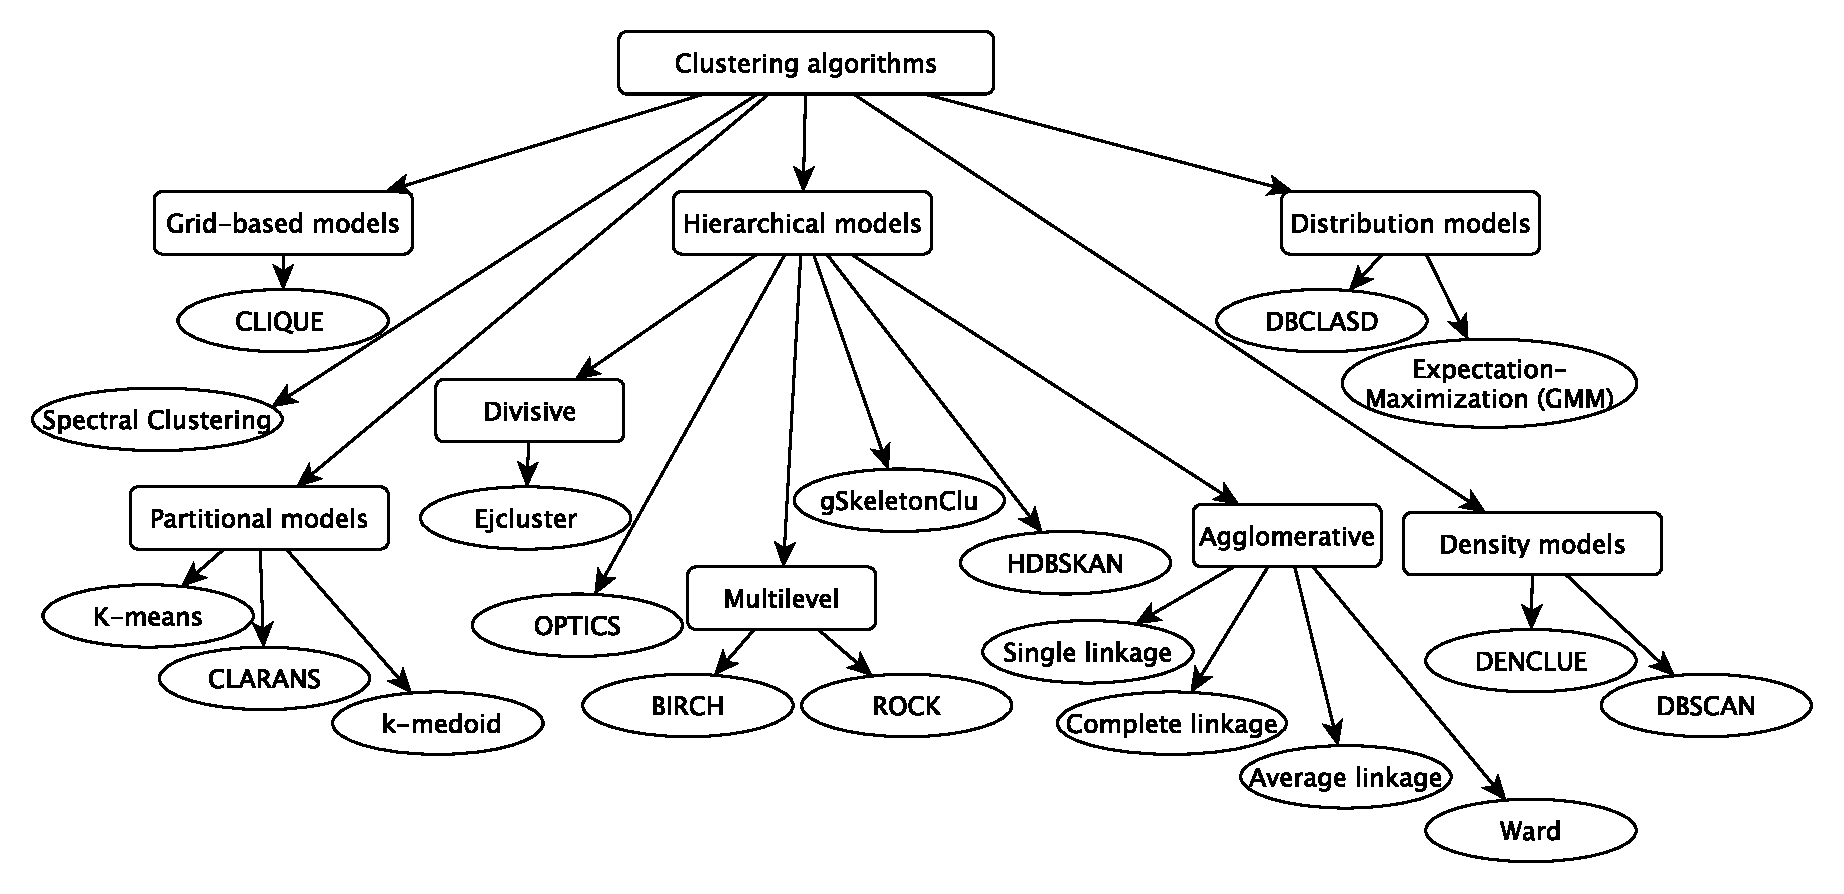
\includegraphics[width=1.0\textwidth]{Fig19.pdf}
    \caption{Taxonomy of cluster analysis techniques.}
    \label{fig:Fig19}
\end{figure}

\section{Cluster Analysis}
\label{Cluster Analysis}
Cluster analysis is a set of unsupervised machine learning techniques aimed at grouping similar in some sense objects together (in clusters). There are many ways to categorize clustering techniques based on the particular underlying approaches. One of the possible taxonomies for some techniques is depicted on~\autoref{fig:Fig19}which is partially based on a number of research on the comparison of different clustering techniques~\cite{steinbach2004challenges}~\cite{karypis2000comparison}~\cite{DBSCANvsK-Means}. Instead, the intention is to cluster financial network participants according to some attributes as good as possible. Generally, a good clustering method will produce high-quality clusters characterised by high intra-class similarity, low inter-class similarity and by some other common clustering quality evaluation metrics.

\subsection{$k$-means}
\label{k-means}
$k$-means is one of the most simple yet effective and common partitioning algorithms for solving a clustering problem in an unsupervised manner. The presumably first description of the technique dates back to 1967~\cite{k-maens1967}. It is an iterative algorithm that seeks local maxima through a sequence of iteration. $k$-means is comparatively fast technique capable of handling large data sets with the linear time complexity. However, like many other clustering techniques, it suffers from "curse of dimensionality".

The starting point and at the same time the most ambiguous step of the algorithm is determining the number of clusters hidden intrinsically in the original data. The initially chosen number could be optimized later based on elbow criterion~\cite{ElbowMethod2014}. For $k$ clusters assign randomly the cluster centroids in the data space~\autoref{fig:Fig20}.
\begin{figure}[H]
    \centering
    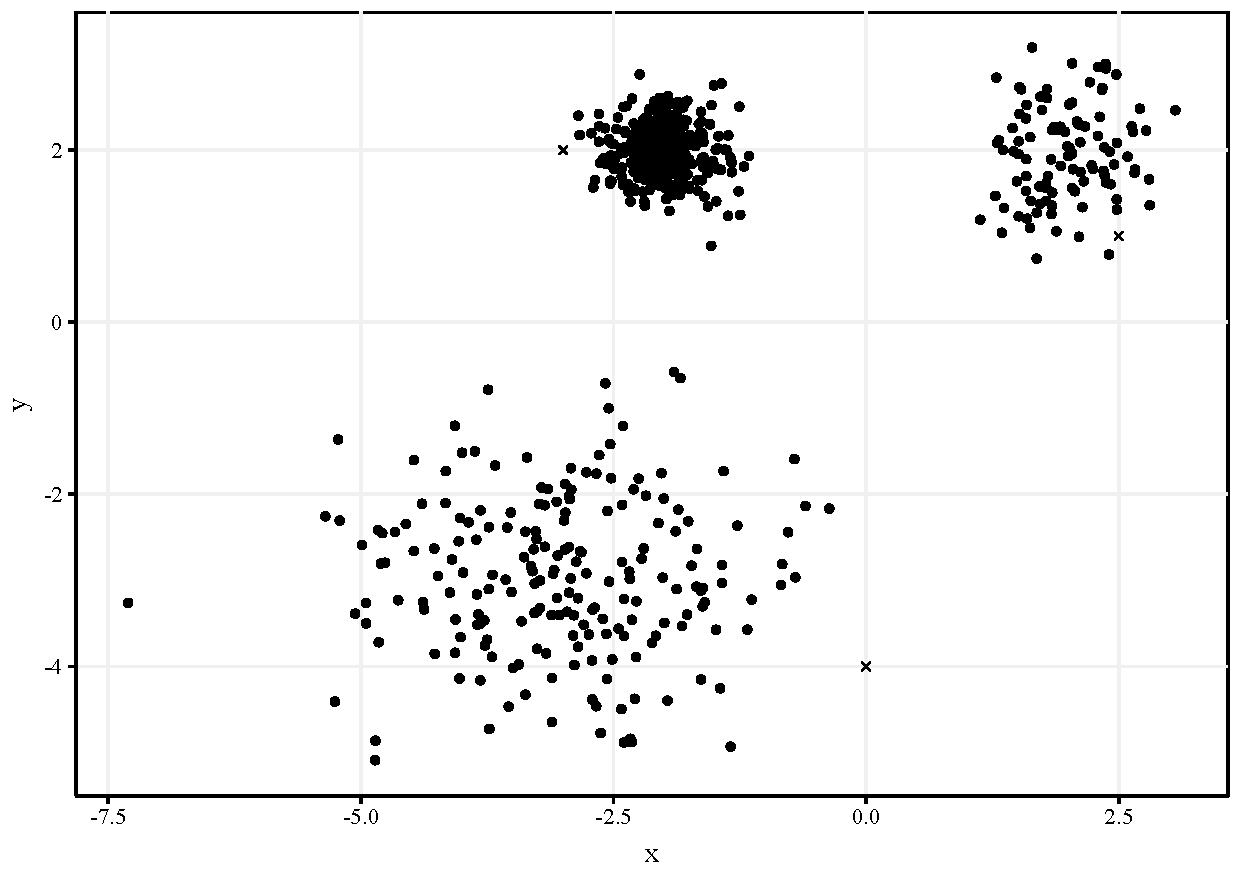
\includegraphics[width=0.65\textwidth]{Fig20.pdf}
    \caption{$k$-means clustering in 2-dimensional space. In the first iteration, the cluster centroids are randomly picked points in the space denoted by crosses on the plot.}
    \label{fig:Fig20}
\end{figure}
The next crucial step of the algorithm is to choose a proper distance measure in the given space. The common choice is to consider the Euclidean distance in a metric space. The Euclidean distance between points $\textbf{x}=(x_1,x_2,...,x_n)$ and $\textbf{y}=(y_1,y_2,...,y_n)$ in Euclidean $n$-dimensional space is defined as follows:

\begin{equation}
  d(\textbf{x,y})=\sqrt{(x_1-y_1)^2+(x_2-y_2)^2+...+(x_n-y_n)^2}
  \label{eq:equat14}
\end{equation}
Unfortunately, if the original space comprises too many dimensions, a pairwise distance ~\autoref{eq:equat10} involves an increasing number of addends under the square root and after its extraction leads to pretty much similar distances between all points in the space - an implication of the "curse of dimensionality". To overcome this flaw it is recommended to reduce the dimensionality of the space before clustering as described in \ref{Dimensionality Reduction}.

The next step is to assign the data points to one of the clusters. The affiliation to the cluster is measured by the distance between a point and a cluster centroid. The smallest distance to a centroid indicates the point's cluster at the current iteration. Once all points are assigned to some cluster, recompute new cluster centroids as the centre of mass among cluster members. Start the next iteration by placing new centroids and repeat the procedure again until the location of centroids will minimize the sum of squared distances from the cluster points~\autoref{fig:Fig21}.
\begin{figure}[H]
    \centering
    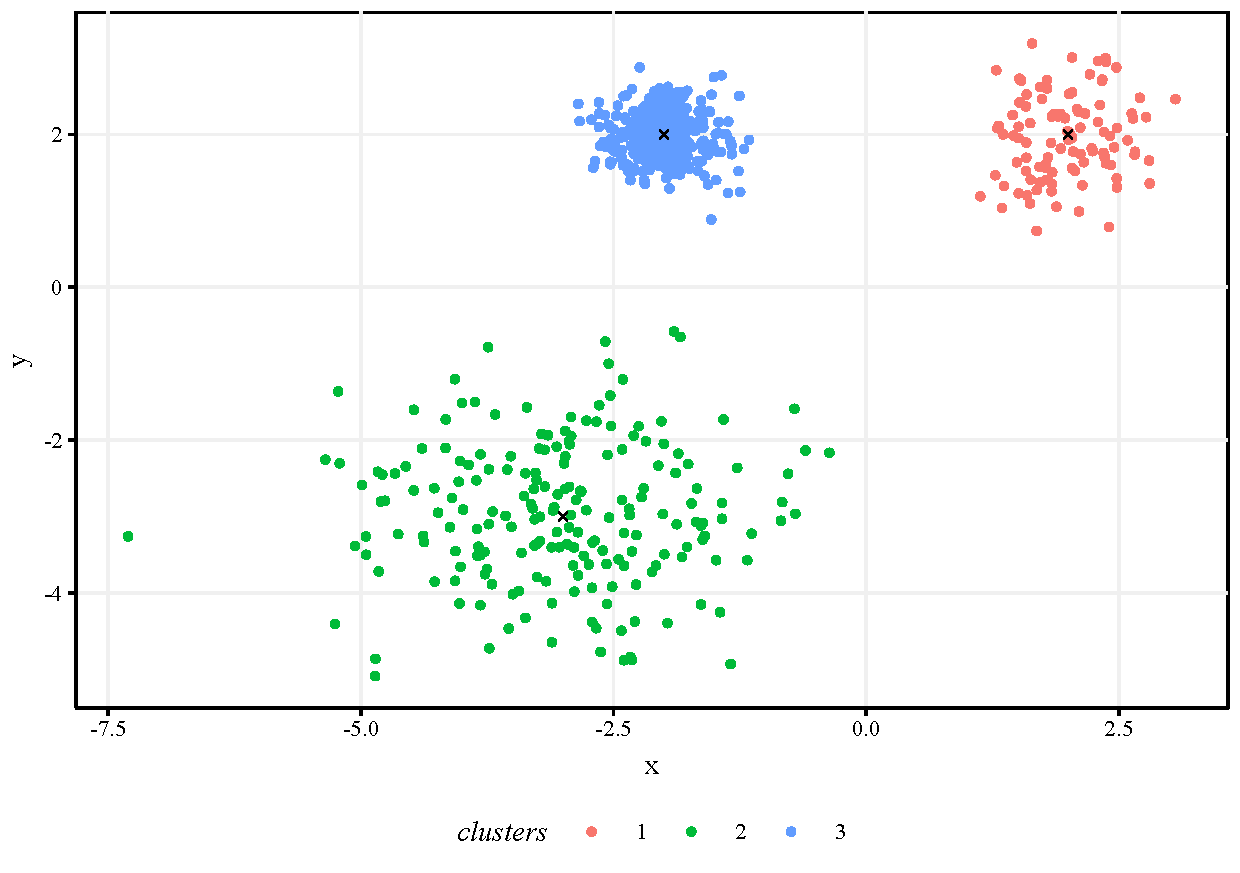
\includegraphics[width=0.65\textwidth]{Fig21.pdf}
    \caption{$k$-means clustering in 2-dimensional space. At the first iteration, the cluster centroids are randomly picked points in the space denoted by crosses on the plot.}
    \label{fig:Fig21}
\end{figure}

The ultimate goal of $k$-means clustering is to minimize total intra-cluster variance. Therefore the objective is represented by the squared error function and looks as follows:
\begin{equation}
  C = \sum_{j=1}^{k} \sum_{i=1}^{n}||x_i^{(j)}-c_j||^2
  \label{eq:equat15}
\end{equation}
where $k$ is a number of clusters, $n$ is a number of data points, and $c_j$ is a centroid of cluster $j$. The optimal number of clusters $k$ assures the best data points separation and minimizes $C$.

In practice, there is usually no prior information about the magnitude of $k$. However, the optimal value could be approximated by comparing the outcomes of multiple runs setting with different $k$. A run with the smallest $C$ usually accounts for the best $k$. It's crucial to treat large values of $k$ carefully. Although they may seem like the best choice in terms of decreasing the error $C$, they often increase the risk of overfitting.

\textbf{Limitations. }
The considerable challenge in $k$-means clustering in practice is a preliminary choice of the number of clusters assumed in the original data. There is no solid theoretical approach to define the optimal number of clusters, nevertheless, there are some methods in practice that may help. The elbow method described in ~\cite{ElbowMethod2014} focuses on  the percentage of variance explained as a function of the number of clusters. The idea of the method is to increment $k$ until adding one more cluster doesn't lead to much better modelling of the data. ~\autoref{fig:Fig22} shows the elbow plot for data points from ~\autoref{fig:Fig21}. The first three clusters along the $x$ axis add the most of information but further increasing does not contribute much. Thereby, the angle ("elbow") formed at the third cluster is considered the optimal point to derive $k$. 

\begin{figure}[H]
    \centering
    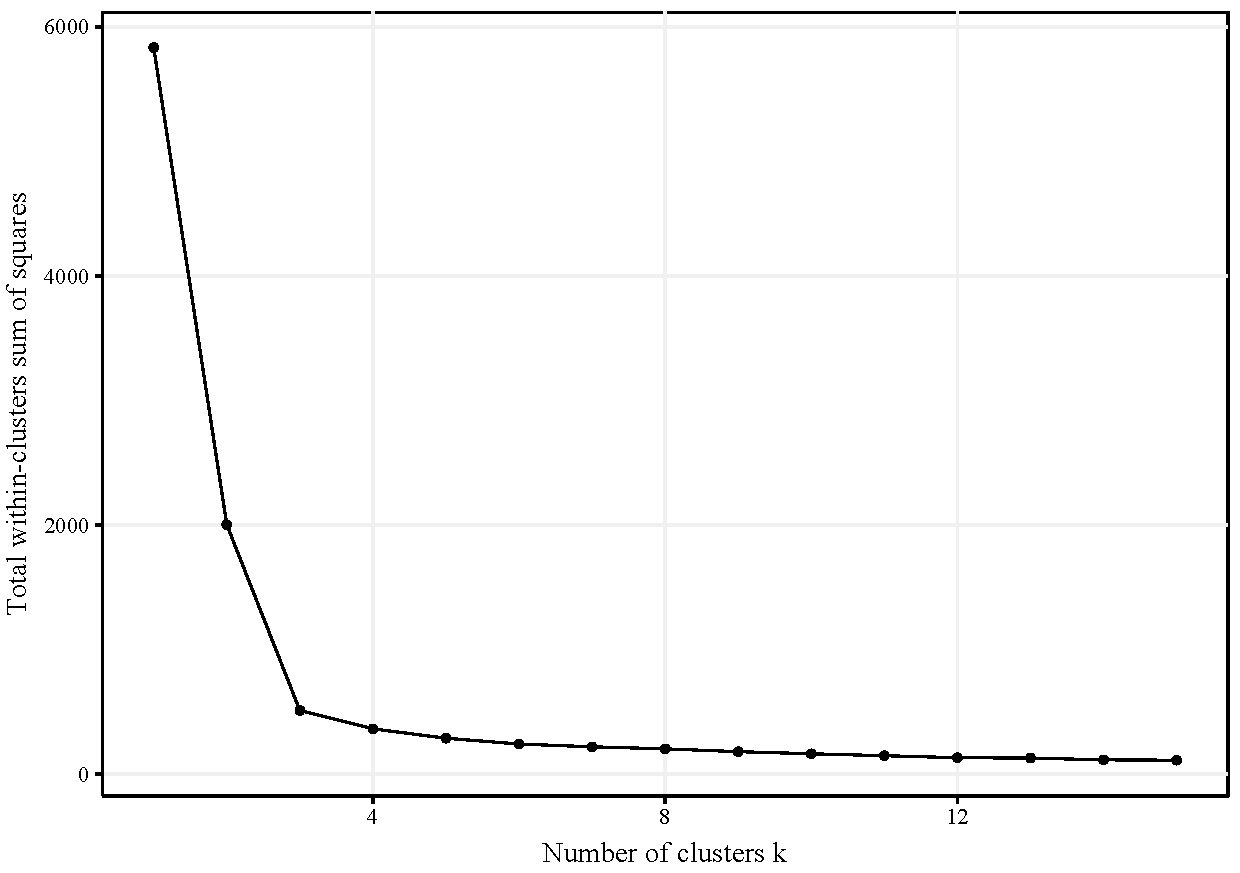
\includegraphics[width=0.5\textwidth]{Fig22.pdf}
    \caption{Elbow plot for the data points from ~\autoref{fig:Fig21}. Three clusters are the optimal choice for the data set.}
    \label{fig:Fig22}
\end{figure}

$k$-means clustering is the stochastic algorithm as the initial centroids are placed at random. Even under preserving the same number of clusters, the algorithm may lead to different outcomes. It is especially common for real-world data. The problem of stability of $k$-means clustering is explored among others in ~\cite{ClusterStability2007}. The common way to identify the stable clusters in practice is to run clustering multiple times and choose the most frequent separation.

Another weakness of the method is an assumption of certain cluster shape (e.g. hyper spherical in a metric space with Euclidean distance). $k$-means is incapable to find bent, S-shaped clusters, or rings.

\subsection{Hierarchical DBSCAN}
Density-Based Spatial Clustering of Applications with Noise in 1996 ~\cite{DBSCAN} in contrast to $k$-means is designed to discover clusters of arbitrary shape. Similar to $k$-means it allows any distance metric, is efficient for large data sets and requires two user-defined input parameters: a maximum radius of the local neighbourhood $Eps$ and a minimum number of points fall in the neighbourhood $MinPts$ that can be reduced to the only last. A density-based notion from ~\cite{DBSCAN} defines a cluster as a maximal set of density-connected points. The significant advantage over $k$-means is that there is no need to set a number of clusters a priori. DBSCAN produces clusters based on the intrinsic structure of the original data.

Hierarchical DBSCAN is a DBSCAN extension first proposed in 2013 ~\cite{HDBSCAN}. Unlike DBSCAN generalization of parameters $Eps$ and $MinPts$ over all clusters, HDBSCAN allows finding clusters of varying densities by performing DBSCAN over varying $Eps$ values and subsequent result integration. This also leads to a more robust parameter selection and overall cluster stability. 

DBSCAN is not hierarchical and finds only "flat" clusters, while density-based hierarchical algorithms like HDBSCAN and OPTICS~\cite{OPTICS1999Ankerst} produce a nested cluster hierarchy. In the case of the second, it creates a cluster-ordering corresponding to many density-based clusterings according to a broad range of parameter settings and then applies a global cut/density threshold to produce "flat" clusters. This strategy may not result in the optimal set of clusters characterized by different density levels.

The main innovation introduced by HDBSCAN creators in~\cite{HDBSCAN} is an automatic method to extract a flat clustering solution based on local cuts applying to a single-linkage-like dendrogram tree in hierarchical clustering in order to extract the most significant clusters. HDBSCAN aims at finding stable clusters by optimizing an objective function to retrieve a global optimum for stability.

The algorithm starts with the assumption of having noise in real data that typically reside in areas of low density. The simplest and parsimonious way to distinguish clusters of higher density from sparsely distributed noise is to consider a distance between the $k$ nearest neighbours in a metric space. Assume $k$ = 5 neighbours surrounding a source point in a metric space, then the \textit{core distances} of randomly chosen points $a$ and $b$ are $core_{k=5}(a)=r1$ and $core_{k=5}(b)=r2$ respectively (~\autoref{fig:Fig23}).

\begin{figure}[H]
    \centering
    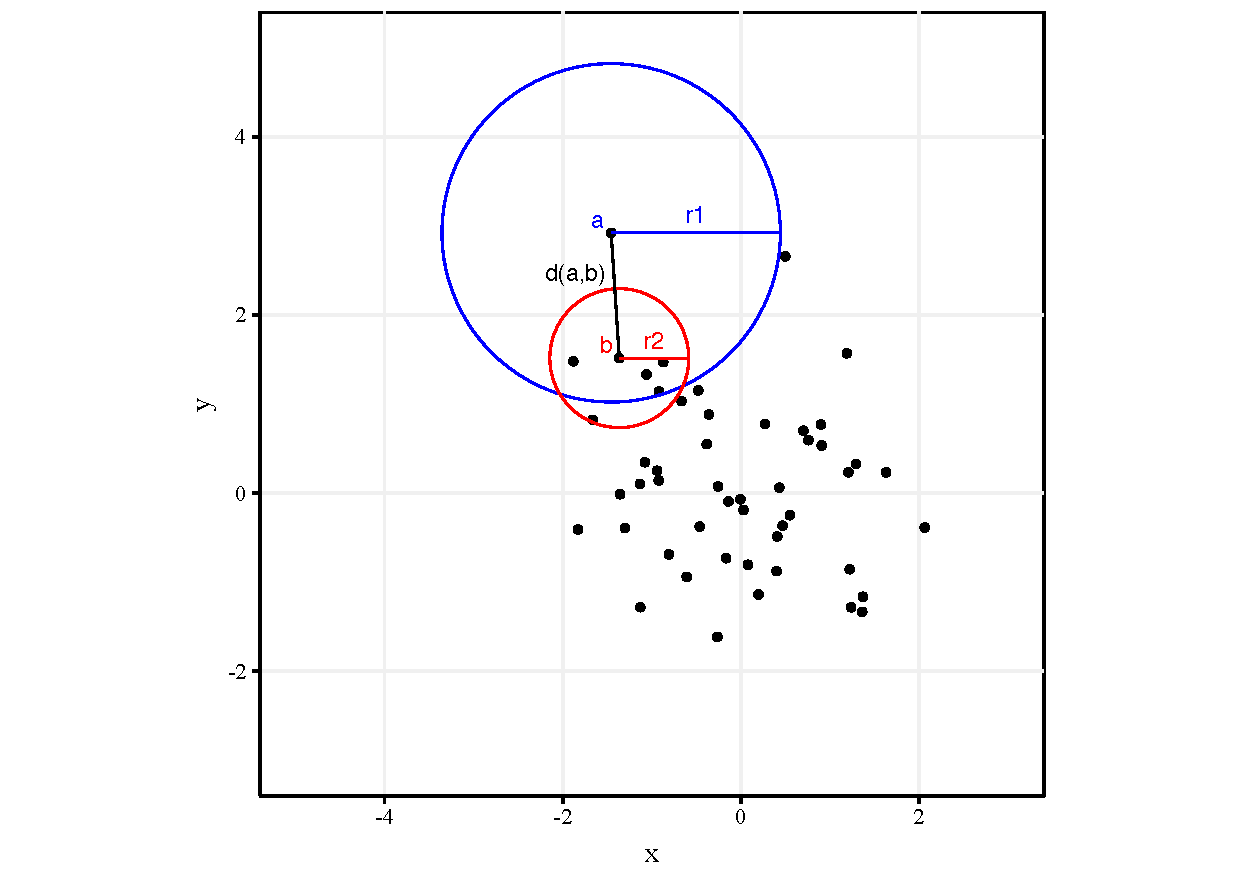
\includegraphics[width=0.55\textwidth]{Fig23.pdf}
    \caption{Core distance of a point is the radius of circumference spanning 5 nearest neighbours with the centre in the source point.}
    \label{fig:Fig23}
\end{figure}

To spread apart points of potential clusters and noise Ricardo J. G. B. Campello et al. proposed to use a \textit{mutual reachability distance}, which is defined for $a$ and $b$ from~\autoref{fig:Fig23} as follows:
\begin{equation}
  d_{m_r_d}(a,b)=max\{core_{k}(a), core_{k}(a), d(a,b)\}
  \label{eq:equat16}
\end{equation}
where $d(a,b)$ is the original metric distance between $a$ and $b$.~\autoref{eq:equat16} suggests preserving the original distance between densely placed points which core distances are smaller than pairwise and this way pushing away sparser points while increasing the pairwise distance to the largest core distance. Therefore, the point $a$ from~\autoref{fig:Fig23} will be pushed away from the denser cluster because $d_{m_r_d}(a,b) = core_{k}(a)$. This approach results in the enlarging margins around dense clusters, however, the choice of $k$ should be prudent: the larger magnitudes lead to more points on cluster borders will be considered as noise.

The next step is to derive the minimum spanning tree of the weighted graph where vertices are data points and an edge between any two points has weight equal to its mutual reachability distance~\autoref{fig:Fig24b}. A complete graph has $n^2$ edges which makes it slow to process while searching for a minimal set of edges connecting all nodes. One of the efficient algorithms for retrieving spanning tree from a connected graph is a Prim–Jarník greedy algorithm\footnote{\textbf{Prim–Jarník algorithm} finds a subset of the edges that forms a tree that includes every vertex where the total weight of all the edges in the tree is minimized. Source: https://www.wikipedia.org}. It finds a minimum spanning tree for a weighted undirected graph and was proposed in 1930 by Vojtěch Jarník~\cite{Jarnik1930SpanningTree} and later rediscovered by Robert C. Prim in 1957~\cite{Prim1957SpanningTree}.

\begin{figure}[H]
    \centering
    \begin{minipage}{0.42\textwidth}
        \centering
        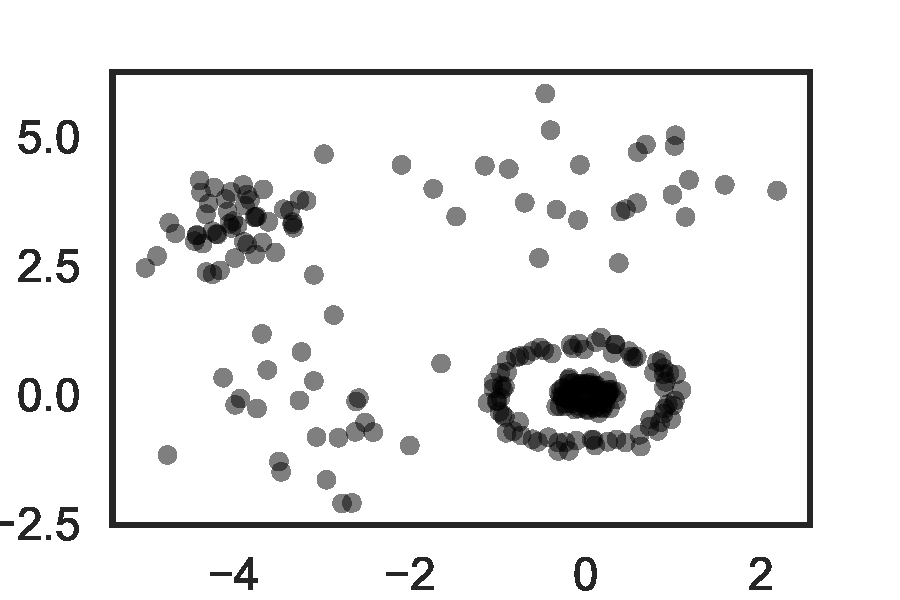
\includegraphics[width=0.9\textwidth]{Fig24a.pdf}
        \caption{Points in the original space.}
        \label{fig:Fig24a}
    \end{minipage}\hfill
    \begin{minipage}{0.42\textwidth}
        \centering
        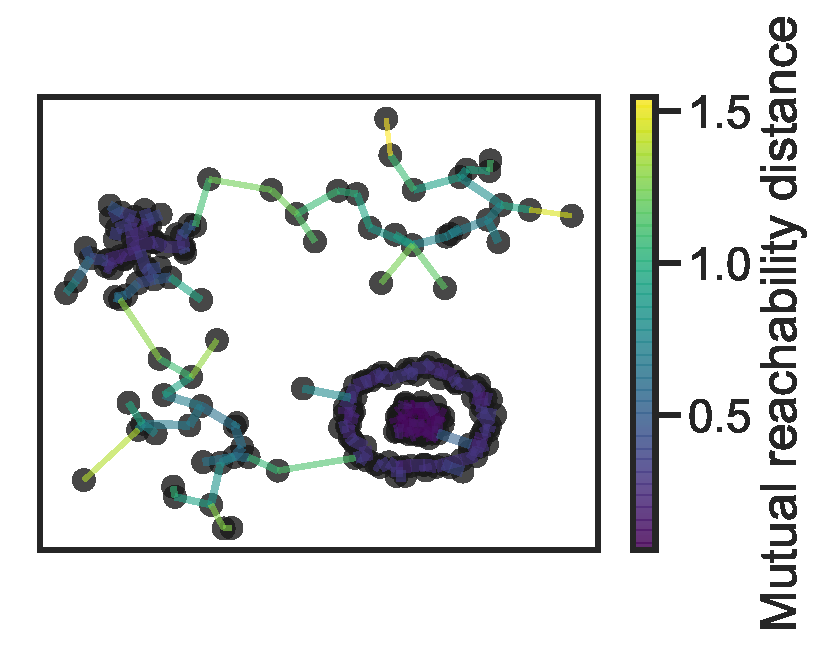
\includegraphics[width=0.9\textwidth]{Fig24b.pdf} 
        \caption{Minimum spanning tree of weighted graph.}
        \label{fig:Fig24b}
    \end{minipage}
\end{figure}
\begin{figure}[H]
    \centering
    \begin{minipage}{0.42\textwidth}
        \centering
        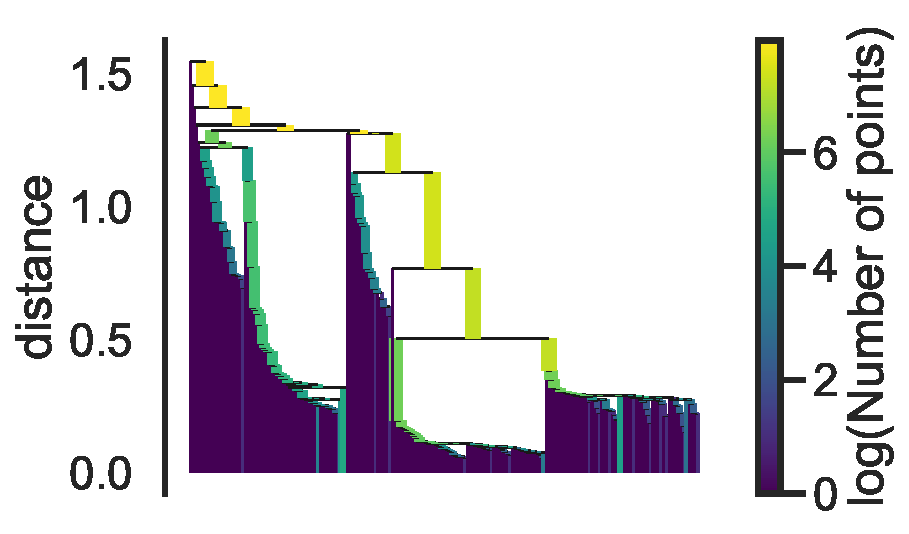
\includegraphics[width=0.9\textwidth]{Fig24c.pdf}
        \caption{Hierarchical dendrogram on mutual reachability distance.}
        \label{fig:Fig24c}
    \end{minipage}\hfill
    \begin{minipage}{0.42\textwidth}
        \centering
        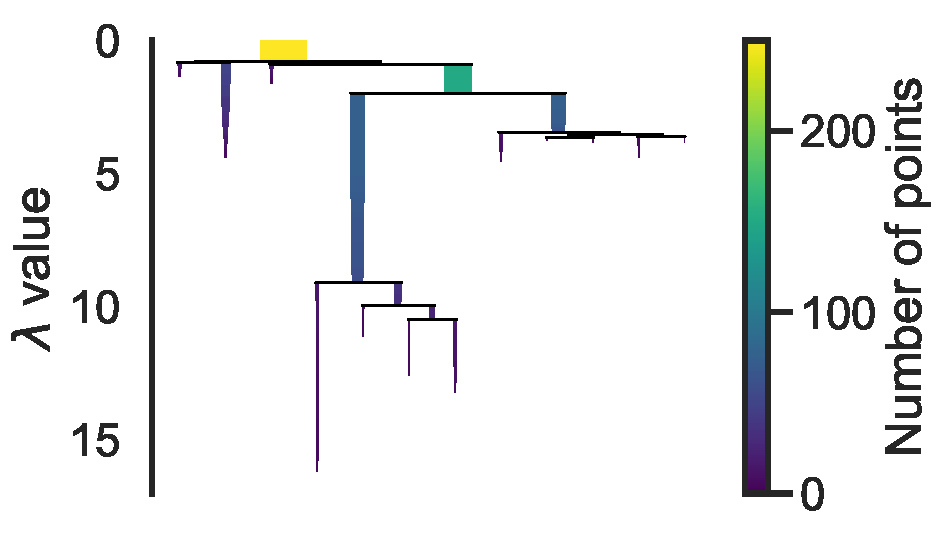
\includegraphics[width=0.9\textwidth]{Fig24d.pdf} 
        \caption{Condensed dendrogram tree without noise points (k = 5)}
        \label{fig:Fig24d}
    \end{minipage}
\end{figure}

A minimum spanning tree serves for producing a cluster hierarchy in the form of a dendrogram~\autoref{fig:Fig24c}. The next intuitive step is to infer a set of flat clusters from a dendrogram. A vast majority of hierarchical clustering techniques suggest determining a single horizontal cut level~\cite{DBSCAN}~\cite{OPTICS1999Ankerst}. However, a global cut on a single density level does not guarantee the best separation among clusters of variable density. 

To distinguish clusters points from noise, HDBSCAN algorithm relies on the user-defined parameter \textit{minimum cluster size}. It facilitates clusters search in the dendrogram: if a number of points falls apart from a cluster lower than minimum cluster size, they will be considered as noise instead of an independent cluster. On the other hand, if a split divides the cluster into two of size exceeding or equal to minimum cluster size, the split is considered as a true cluster split. This heuristic is used to truncate the dendrogram tree by eliminating noise points. After traversing the tree, the only clusters of the sufficient size persist and the rest of the points are discarded. This makes original dendrogram tree thinner like on~\autoref{fig:Fig24d} where minimum cluster size $k$=5. Here the width of the lines represents the number of points in the cluster and the pointed leaves show when noise points fall out of the clusters over the increase of mutual reachability distance.

The innovative part of the algorithm is a heuristic on an unequivocal choice of stable, long-lived, "flat" clusters. For each point of each cluster in a condensed tree on ~\autoref{fig:Fig24d} assume $\lambda_p=\frac{1}{distance_p}$ equal to reciprocal of mutual reachability distance at which that point fell out of the cluster. Additionally, for each cluster assume $\lambda_{birth}$ and $\lambda_{death}$ are equal to reciprocals of mutual reachability distance when a new cluster splits off from its parent and when a cluster splits into smaller clusters respectively. For a particular cluster $\lambda_{birth}< \lambda_p <\lambda_{death}$ and its cluster stability measure is calculated as follows:

\begin{equation}
  S = \sum_{p\in cluster}(\lambda_p - \lambda_{birth})
  \label{eq:equat17}
\end{equation}
The measure is calculated for each cluster bottom-up starting with the leaf-clusters. If the sum of the stabilities of the child clusters surpluses parent stability, then assign this sum to the parent stability. Otherwise, if the parent stability is greater than the sum of its children stabilities, then include this cluster in the final set of "flat" clusters and exclude all its descendants. Continue the process until reaching the root, then traverse tree top-down and collect the selected "flat" clusters as ~\autoref{fig:Fig25} illustrates.
\begin{figure}[!hp]
    \centering
    \begin{minipage}{0.42\textwidth}
        \centering
        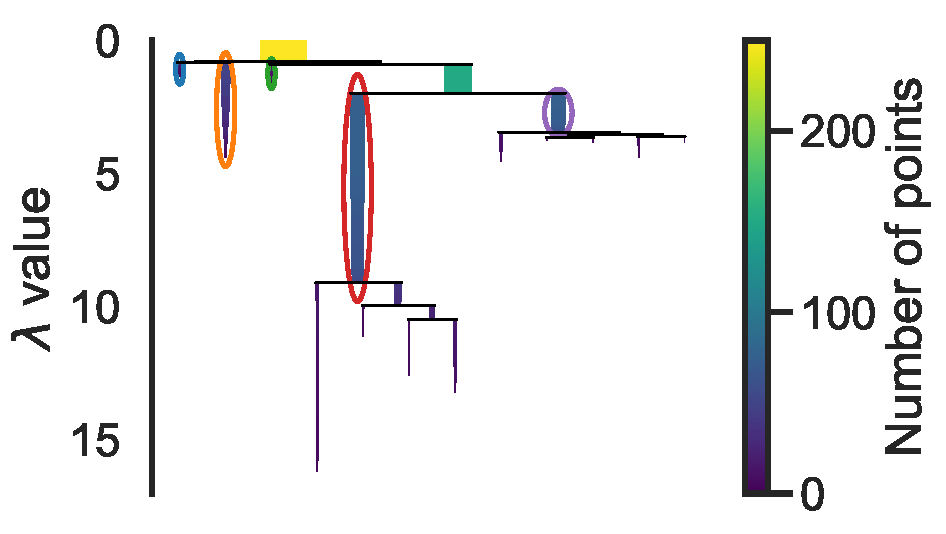
\includegraphics[width=0.9\textwidth]{Fig25.pdf}
        \caption{Selected "flat" clusters in the condense tree.}
        \label{fig:Fig25}
    \end{minipage}\hfill
    \begin{minipage}{0.42\textwidth}
        \centering
        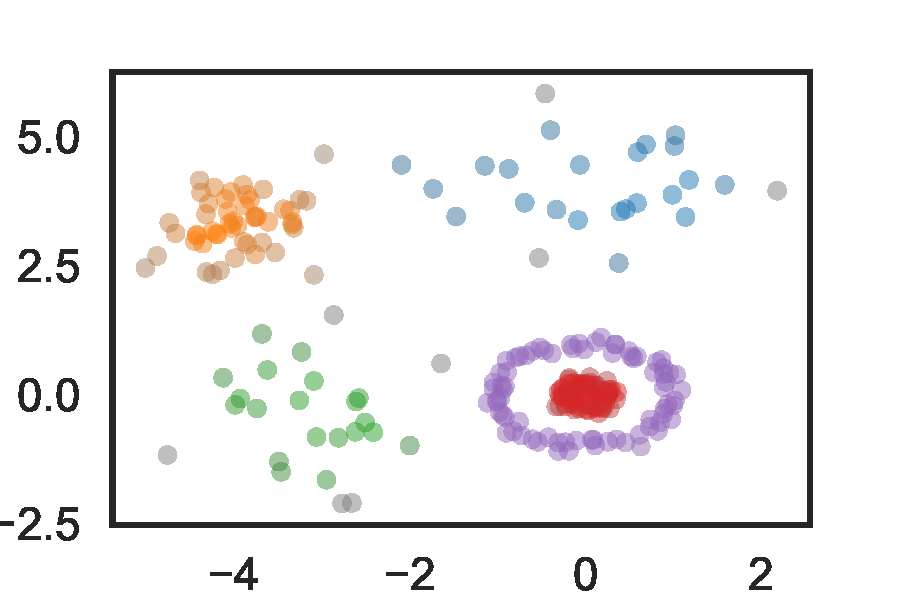
\includegraphics[width=0.9\textwidth]{Fig26.pdf} 
        \caption{Points labelled by HDBSCAN-defined cluster membership.}
        \label{fig:Fig26}
    \end{minipage}
\end{figure}

The result on ~\autoref{fig:Fig26} demonstrates that the proposed density-based hierarchical clustering algorithm is capable to find clusters of varying density along with clusters of arbitrary shapes like a ring and distinguish them from detached noise points.

\section{Cluster evaluation strategies}
\label{Cluster evaluation strategies}
A clustering evaluation relies on assessment measures, which serve for comparing results from different clustering algorithms on one scale. The clustering evaluation is needed to compare two or more clustering algorithms, tune clustering hyperparameters and to avoid finding clusters in random data. Generally, clustering evaluation statistics are divided between two classes: internal and external. Internal measures use only internal information on clustered data to evaluate the goodness of clustering, while external measures rely on externally provided ground truth labels. This section will discuss several internal clustering evaluation measures for unsupervised clustering.

\begin{enumerate}
  \item \textit{Root-mean-square standard deviation index (RMSSTD)}~\cite{sharma1996RMSSDT} measures the homogeneity of the clusters. In essence, it is a square root of the pooled sample variance of all variables.
      \begin{equation}
    RMSSTD = \sqrt{\frac{SS_1+...+SS_p}{df_1+...+df_p}}\;,\;\;\; where\;SS_j = \sum_{i=1}^{n}(x_{ij}- \boldsymbol{x_j} )^2
    \label{eq:equat18}
    \end{equation}
  where $p$ is a number of clusters, $SS_j$ is the within sum of squares of the $j$-th variable. The low RMSSTD values testify the high within-clusters homogeneity and hence a better clustering.
  
  \item \textit{R-square index (RS)}~\cite{sharma1996RMSSDT} measures the extent to which clusters are different from each other. It is a ratio of the difference between the total sum of squares and the total between sum of squares to the total sum of squares.
    \begin{equation}
    RS = \frac{SS_{total}-SS_{within}}{SS_{total}}\;,\;\; where\;SS_{total}=\sum_{j=1}^p \sum_{i=1}^n (x_{ij}-\boldsymbol{x_j})^2
    \label{eq:equat19}
    \end{equation}
  The minimum RS value 0 means there is no difference among the clusters, the maximum value 1 indicates a significant difference among the clusters.
  
  \item \textit{SD Validity index (SD)}~\cite{halkidi2000quality} relies on the average scattering of clusters and total separation of clusters. The scattering is calculated as the ratio of within-cluster variances to the variance of the data set, while the total separation of clusters is based on the distance between cluster centres $c_i$:
    \begin{equation}
        Scatt = \frac{1}{p}\sum_{i=1}^p \frac{||\boldsymbol{\sigma(c_i)}||}{||\boldsymbol{\sigma(x)}||}\;,\;\;\; Dis = \frac{\max_{i,j=1...p}||c_j-c_i||}{min_{i,j=1...p}||c_j-c_i||}\sum_{k=1}^p \bigg(\frac{1}{\sum_{\substack{j=1 \\ i\neq j}}^p ||c_j-c_i||}\bigg)
    \label{eq:equat20}
    \end{equation}
    \begin{equation}
        SD = Dis_{maximal\;p} \cdot Scatt + Dis
    \label{eq:equat21}
    \end{equation}
    The low SD Validity index values means better clustering: clusters are compact and well separated.
    
  \item \textit{S\_Dbw Validity index (S\_Dbw)}~\cite{halkidi2001S_Dbw} is based on cluster compactness and separation and, additionally, considers clusters densities. The intra-cluster variance is $Scatt$ from ~\autoref{eq:equat20}, and the inter-cluster density is defined as follows:
      \begin{equation}
        Dens\_bw=\frac{1}{p(p-1)}\sum_{i=1}^p \Big(\sum_{\substack{j=1 \\ i \neq j}}^p \frac{density(u_{ij})}{\max\{density(c_i),density(c_j)\}}\Big)
    \label{eq:equat22}
    \end{equation}
  where $u_ij$ is the middle point between clusters centres $c_i$ and $c_j$. The $density$ function counts the number of points in a hyper-sphere with radius equal to the average standard deviation of clusters ($avg\_std\_clus = \frac{1}{p}\sqrt{\sum_{i=1}^p||\sigma(c_i)||}$ ).
    \begin{equation}
        S\_Dbw=Scatt+Dens\_bw
    \label{eq:equat23}
    \end{equation}  
  It enables reliable evaluation of globular clusters. Low $S\_Dbw$ values indicate a good clustering result. 
  
  \item \textit{Silhouette coefficient (SC)}~\cite{zhu2010clustering} is a measure of how similar an object is to its own cluster compared to other clusters. The coefficient is relevant for hierarchical and partitioning clustering techniques.
    \begin{equation}
    SC = \frac{1}{n}\sum_{i=1}^n \frac{b_i - a_i}{\max\{a_i, b_i\}}
    \label{eq:equat24}
    \end{equation}
  where $a_i$ is the average distance between $i$ and all other data points in the same cluster and $b_i$ is the smallest average distance of $i$ to all points in any other cluster, of which $i$ is not a member.
      \begin{equation}
        a_i = \frac{1}{|C_i|-1}\sum_{j=C_i,i\neq j} d(i,j)\;\;\;\;\; 
        b_i = \min_{i\neq j} \frac{1}{|C_i|}\sum_{j\in C_j} d(i,j)
        \label{eq:equat20}
      \end{equation}
  where $d(i,j)$ is the distance between data points $i$ and $j$ in the cluster $C_{i}$. The SC value may vary between -1 and 1. The higher values characterizes better clustering.
  
  \item \textit{Davies–Bouldin index (DB)}~\cite{davies1979cluster} is an internal, very fast comparing to Silhouette coefficient evaluation measure calculated as follows:
    \begin{equation}
        DB = \frac{1}{|C_i|-1}\sum_{j=C_i,i\neq j} d(i,j)
        \label{eq:equat21}
     \end{equation}
  where $n$ - the number of clusters, $c_{x}$ - the centroid of cluster $x$, $\sigma _{x}$ - the average distance from all elements in the cluster $x$ to centroid $c_{x}$, and $d(c_{i},c_{j})$ - the distance between centroids $c_{i}$ and $c_{j}$.
  
  \item \textit{Dunn index (D)}~\cite{Dunn1973index} tends to identify dense and well-separated clusters by dividing the minimal inter-cluster distance by the maximal intra-cluster distance:
    \begin{equation}
        D = \frac{\min_{1\leqslant i < j \leqslantn n}d(i,j)}{\max_{1\leqslant k\leqslant n}d'(k)}
        \label{eq:equat22}
     \end{equation}  
    where $d(i,j)$ - the distance between clusters $i$ and $j$, $d'(k)$ - the intra-cluster distance of cluster $k$. Clusters with high intra-cluster similarity and low inter-cluster similarity increases Dunn index.
    
    \item \textit{Calinski-Harabasz index}~\cite{CH2007} is higher when clusters are dense and well separated. For $k$ clusters, the Calinski-Harabasz score $CH$ is given as the ratio of the between-clusters dispersion mean and the within-cluster dispersion:
        \begin{equation}
            CH(k) = \frac{Tr(\boldsymbol{B_k})}{Tr(\boldsymbol{W_k})} \times \frac{N-k}{k-1}
            \label{eq:equat23}
         \end{equation}
     where $N$ is the number of the data points, $\boldsymbol{B_k}$ is the between-clusters dispersion matrix and $\boldsymbol{W_k}$ is the within-cluster dispersion matrix defined as:
        \begin{equation}
            \boldsymbol{B_k} = \sum_q n_q(c_q-c)(c_q-c)^T\;\;\;\; \boldsymbol{W_k} = \sum_{q-1}^k \sum_{x \in C_q} (x-c_q)(x-c_q)^T
            \label{eq:equat24}
        \end{equation}
    with $C_q$ - the set of points in cluster $q$ , $c_q$ - the center of cluster $q$, $c$ - the center of dataspace $E$, and $n_q$ - the number of points in cluster $q$.
\end{enumerate}

\section{Financial Networks}
\label{Financial Networks}
During the last decades, a concept of financial network has been actively exploited for studying the rapidly evolving global interconnected financial system. The major areas where the concept has already proved its utility are financial contagion and systemic risk~\cite{ContagionFinNets} ~\cite{ResContagionFinNets} ~\cite{NetStrucSysRiskBankSys}. Such detrimental phenomena as the common shock propagation, the unfolding of default cascades, and the domino effects of insolvency motivated many researchers to use the financial network model to track a spillover effect. Other areas, where the financial networks have recently come into play are stock market analysis~\cite{NetAnalysisChineseStockMarket} ~\cite{StatisticAnalysisFinNetworks}, formation of interbank markets, assessing stability of financial systems, fraud and anomalies detection~\cite{AnomalyNetIntrusion}, and much more.

Unfortunately, there are not so many publicly-available researches exploring real-world transaction data because of the highly sensitive nature of the data. However, the enormous recent popularity of decentralized platforms based on blockchain technology launched fresh incentives in financial networks studies. A great variety of cryptocurrencies attracted attention of many investors due to real-time transparent maintaining of a public digital ledger of transactions, which is considered to be incorruptible~\cite{miraz2018applications}.

This fact spawned a lot of different financial transaction networks built on mutual trust where the value of an asset is defined by supply and demand similar to a state currency in a bank transaction. Some research on characterizing such networks have been recently done all over the world ~\cite{victormeasuring}, ~\cite{BlockchainGraph}, ~\cite{miller2015discovering}.

Despite the lack of publicly available data from financial institutions to dissect financial network phenomena, there are some studies based on real-world data. Comprehensive research of the real-world transaction data disclosed by Bank of Japan in 2004 ~\cite{inaoka2004fractal} detected a fractal structure of the dynamic network formalized from the set of transactions between financial institutions. The behaviour of financial players in Austria was studied in 2009 by exploring a topology of the network, in which accounts are represented as nodes and transactions are weighted edges between the nodes~\cite{Kyriakopoulos2009}.

\section{Summary}
The current chapter covered all existing techniques, that are used in the concept of the thesis. These techniques have been provided with illustrated explanations, known limitations and references to authors and related works. The next chapter gives an understanding how the discussed methods are applied in the context of the current work.
